\documentclass[twocolumn, 10pt]{extarticle}

% Uncomment to squeeze everything onto one side
\usepackage{pgfpages}
\pgfpagesuselayout{2 on 1}[letterpaper, landscape]

\usepackage[letterpaper,margin=0.25in]{geometry}
\input{ncommon}
\everymath{}
\usepackage{titlesec}

% Options: [subtle], [moderate], or [extreme]
\usepackage[extreme, mathspacing=normal, lists=normal]{savetrees} 
% Restore space between operators (sin, cos, log) and variables
% \thinmuskip=3mu       % Readable sin/cos
% \medmuskip=2mu        % Tight + and -
% \thickmuskip=3mu      % Tight =
\usepackage{enumitem} % Needs to come after

\titleformat{\section}
  {\normalfont\fontsize{12}{14}\bfseries}{\thesection}{1em}{}
\titlespacing\section{0pt}{5pt plus 2pt minus 2pt}{2pt plus 1pt minus 1pt}
\titlespacing\subsection{0pt}{5pt plus 2pt minus 2pt}{2pt plus 1pt minus 1pt}
\titlespacing\subsubsection{0pt}{5pt plus 2pt minus 2pt}{2pt plus 1pt minus 1pt}
%\renewcommand{\arraystretch}{1.5}
\setlist{nosep}
\setlength{\abovedisplayskip}{3pt}
\setlength{\belowdisplayskip}{3pt}
\setlength{\parindent}{0pt}
\raggedbottom

\title{ROB501 Exam Aidsheet}
\author{Tyler Tian}

\begin{document}

\section{Intro Lecture}

\textbf{Vision pipeline:} Pre-processing (noise-reduction, image scaling, color space conversion, gamma correction),
selecting areas of interest (object detection, bkgd subtraction, feature/keypt extraction, image segmentation), precise
preocessing of selected regions (obj. recognition, tracking, feature matching), decision making (motion analysis,
match/no match, flag events).

\textbf{Why so difficult}: Vision is an inverse problem. For inv. probs, often have to appeal to prob. models or
assumptions. Many vision probs are ill-posed and have non-unique sol'ns.

\textbf{Well-posed problem:} (1) A sol'n exists, (2) sol'n is unique, (3) sol'n behav. changes cont. w init. conds.

\textbf{Imaging function:} \[I =
\mathcal{P}(\text{Geometry},\text{Materials},\text{Viewpt},\text{Lighting},\text{Atmospherics}, \epsilon)\]
$\mathcal{P}$ is perspective projection. $(G, M, V) = \mathcal{P}^{-1}(I)$ is what we want.

\textbf{A key issue:}
Geometry is 3D (maybe 4D), appearance is 2D projection of this geometry (depends only weakly on geometry).

\textbf{Human vision:} human retina is 576 megapixels, 20-bit dynamic range, foviated vision (2\degree in centre of view
is super high res, rest is meh but brain fills it in).

\textbf{Morevec's paradox:} hard problems (intelligence tests, games) are easy, easy problems (basic perception,
mobility) are hard.

\section{Mathematical Foundations} %%%%%%%%%%%%%%%%%%%%%%%%%%%%%%%%%%%%%%%%%%%%%%%%

\textbf{Homogeneous Coordinates:} \(\tilde{\bm x} = (\tilde x, \tilde y, \tilde w)\in \mathbb P^2\) where
\(\mathbb P^2 = \reals^3\,\backslash\,(0, 0, 0)\) is a \textbf{projective space}. Points with \(\tilde w = 0\) are
\textbf{points at infinity}. \(\bar{\bm x} = (x, y, 1)\) denotes normalized form or \textbf{augmented vector}.

\(\mathbb P^2\) can be thought of as the set of all lines in \(\reals^3\) that pass through the origin. It is
topologically equivalent to the unit sphere as antipodal points are equivalent (points infinitely far away meet at the
centre of an image). Lines in \(\mathbb P^2\) are planes in \(\reals^3\) passing through the origin.

\textbf{Lines in 2D:} \(\tilde{\bm l} = (a, b, c)\) represents \(\bar{\bm x} \cdot \tilde{\bm l} = ax + by + c = 0\).
Normalize as \(\bm l = (\hat n_x, \hat n_y, d) = (\hat{\bm n}, d)\) with normal and distance to origin.
\(\tilde{\bm l}_1, \tilde{\bm l}_2\) intersect at \(\tilde{\bm l}_1 \times \tilde{\bm l}_2\).

\textbf{Skew-Symmetric Form:} \(\bm u \times \bm v = \skewsym{\bm u}\bm v\) where \(\skewsym{\bm u} = -\skewsym{\bm u}^T\)
\[\skewsym{\bm u} = \matthree{0}{-u_3}{u_2}{u_3}{0}{-u_1}{-u_2}{u_1}{0}\]

\textbf{Homogeneous Transformations:} For given \(\bm C, \bm t\):
\[\bm H = \mattwo{\bm C}{\bm t}{\bm 0^T}{1} \quad \bm H^{-1} = \mattwo{\bm C^T}{-\bm C^T\bm t}{\bm 0^T}{1}\]

\subsection{Rotation Representations}

\textbf{Rotation Matrices:} Orthonormal matrices, \(\bm C\bm C^T = \bm C^T\bm C = \bm I\) where \(\bm C \in SO(2)\) or
\(SO(3)\). In 2D, \(\bm C = \mattwo{\cos\theta}{-\sin\theta}{\sin\theta}{\cos\theta}\).

\textbf{Euler Angles:} Begin with aligned frames, perform each rotation about a different intermediate frame axis.
\[
\bm C(\phi) = \matthree{1}{0}{0}{0}{\cos\phi}{-\sin\phi}{0}{\sin\phi}{\cos\phi} \qquad
\bm C(\theta) = \matthree{\cos\theta}{0}{\sin\theta}{0}{1}{0}{-\sin\theta}{0}{\cos\theta}
\]
\[
\bm C(\psi) = \matthree{\cos\psi}{-\sin\psi}{0}{\sin\psi}{\cos\psi}{0}{0}{0}{1}
\]
Yaw-pitch-roll set of Euler angles: \(\bm C(\psi, \theta, \phi) = \bm C(\psi)\bm C(\theta)\bm C(\phi) =\)
\[
\begin{bsmallmatrix}
\cos\psi\cos\theta && \cos\psi\sin\theta\sin\phi - \sin\psi\cos\phi && \cos\psi\sin\theta\cos\phi + \sin\psi\sin\phi \\
\sin\psi\cos\theta && \sin\psi\sin\theta\sin\phi + \cos\psi\cos\phi && \sin\psi\sin\theta\cos\phi - \cos\psi\sin\phi \\
-\sin\theta && \cos\theta\sin\phi && \cos\theta\cos\phi
\end{bsmallmatrix}
\]

\textbf{Axis-Angle:} Rotation by \(\theta\) around \(\hat{\bm n}\). Use \textbf{Rodriguez's formula} to convert to
matrix: \[\bm C(\hat{\bm n}, \theta) = \bm I_3 + \sin\theta\skewsym{\hat{\bm n}} + (1 - \cos\theta)\skewsym{\hat{\bm n}}^2\]

\textbf{Quaternion:} \(\bm q = q_0 + \brm q = q_0 + q_1i + q_2j + q_3k \in \mathbb H\) are normalized to be unit length on \(\mathbb S^3\),
which forms a \textbf{double cover} of \(SO(3)\).
\(\bm q\) is the same rotation as \(-\bm q\). \(\bar{\bm q}\) (conjugate) is the opposite rotation.
Multiply as \[\bm p \otimes \bm q = (p_0 + \bm{\mathrm p}) \otimes (q_0 + \bm{\mathrm q}) = p_0q_0 - \bm{\mathrm p}^T\bm{\mathrm q} + p_0\bm{\mathrm q} + q_0\bm{\mathrm p} + \bm{\mathrm p} \times \bm{\mathrm q}\]

Axis-angle: \(\bm q = \cvec{q_0}{\brm q} = \cvec{\cos(\theta/2)}{\hat{\bm n}\sin(\theta/2)}\).

Rotation matrix: \(\bm C(\bm q) = \bm I_3 + 2q_0\skewsym{\bm{\mathrm{q}}} + 2\skewsym{\bm{\mathrm q}}^2 =\)
\[
\matthreeb{1 - 2q_2^2 - 2q_3^2}{2q_1q_2 - 2q_0q_3}{2q_0q_2 + 2q_1q_3}{2q_0q_3 + 2q_1q_2}{1 - 2q_1^2 - 2q_3^2}{2q_2q_3 - 2q_0q_1}{2q_1q_3 - 2q_0q_2}{2q_0q_1 + 2q_2q_3}{1 - 2q_1^2 - 2q_2^2}
\]

\subsection{Linear Transformations}

\begin{center}
    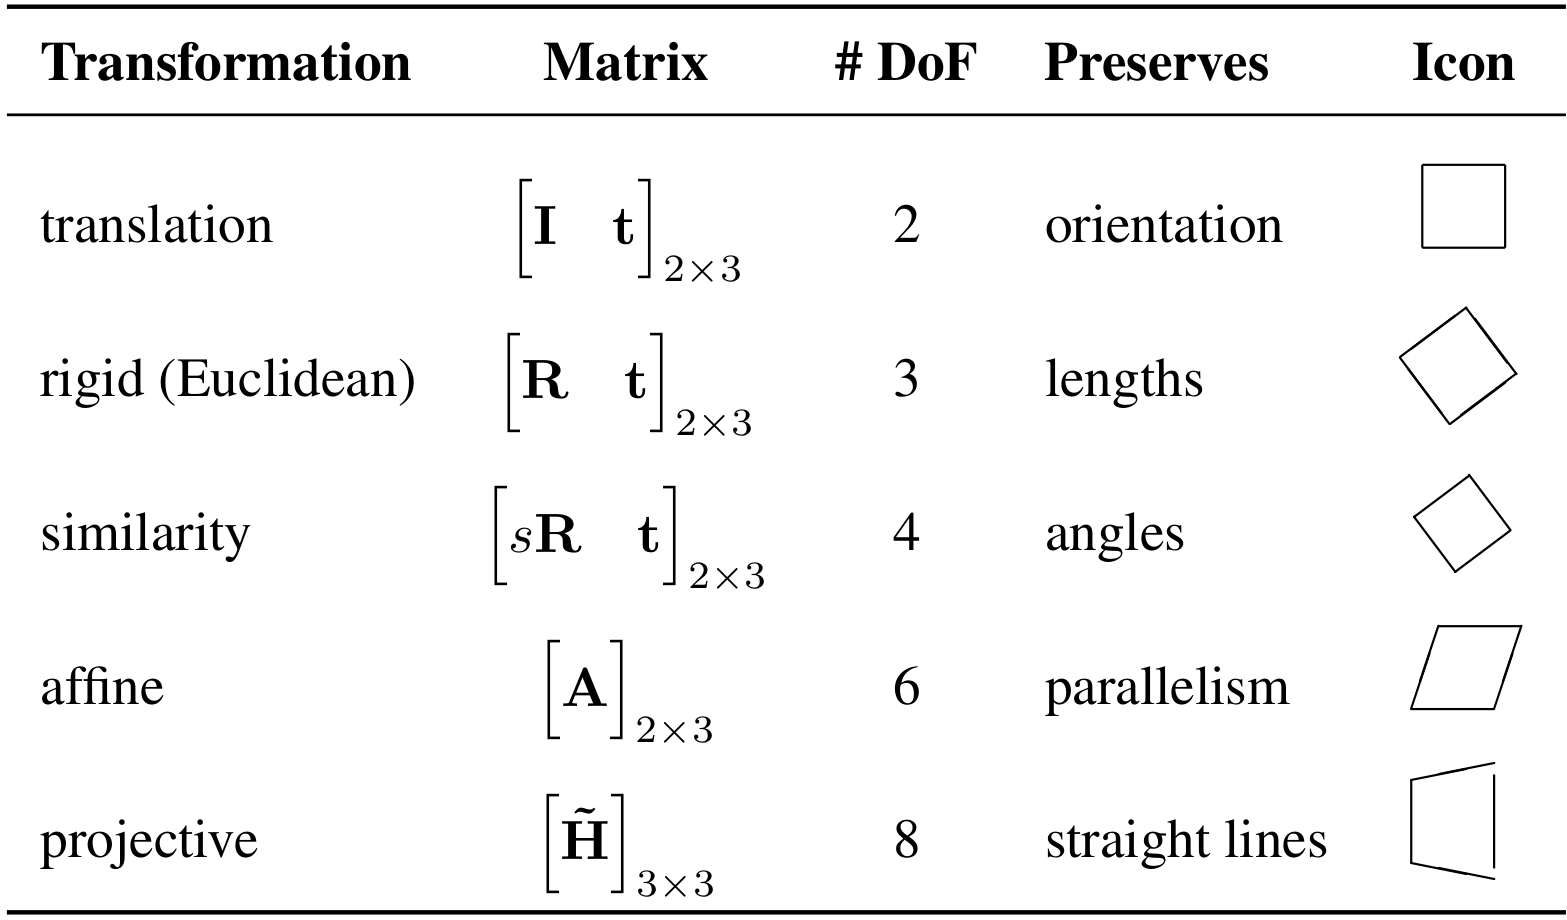
\includegraphics[width=\linewidth]{imgs/2d_transforms.png} \\
    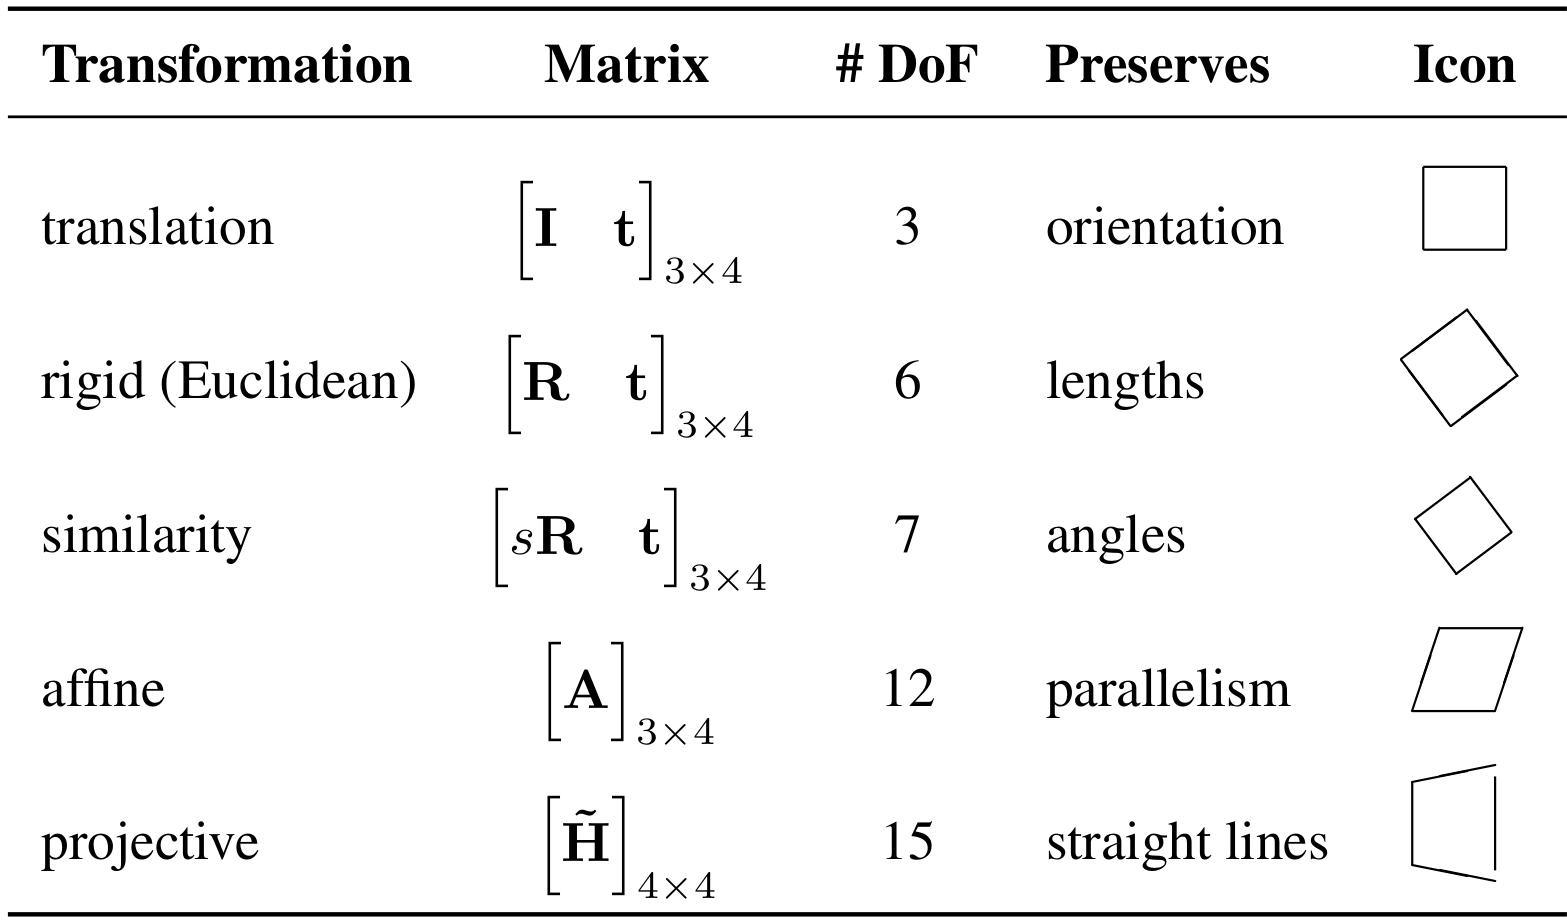
\includegraphics[width=\linewidth]{imgs/3d_transforms.png}
\end{center}

\textbf{Examples:} Camera intrinsic matrix is 2D affine; extrinsic matrix is 3D Euclidean. Perspective projection is
3D projective. Composition of projections is projective.

\section{Probability and Estimation} %%%%%%%%%%%%%%%%%%%%%%%%%%%%%%%%%%%%%%%%%%%%%%%%

\subsection{Probability Definitions}

\textbf{Cumulative Distribution Function:} \(\displaystyle F_x(x) = \sum _{\bar x = -\infty}^x f_x(x)\)

\textbf{Marginalization} and \textbf{Conditioning}:
$$f_x(x) = \sum _{y \in \mathcal Y} f_{xy}(x, y) \qquad f_{x|y}(x|y) = \frac{f_{xy}(x, y)}{f_y(y)}$$
For conditional probabilities:
$$f_{x|z}(x|z) = \sum _{y \in \mathcal Y} f_{xy|z}(x, y|z) \qquad f_{x|y,z}(x|y, z) = \frac{f_{xy|z}(x, y|z)}{f_{y|z}(y|z)}$$

\textbf{Law of Total Probability:} \(\displaystyle f_x(x) = \sum _{y \in \mathcal Y} f_{x|y}(x|y)f_y(y)\)

\textbf{Bayes' Rule:}
$\displaystyle \underbrace{f_{x|y}(x|y)}_{\text{posterior}} = \frac{\overbrace{f_{y|x}(y|x)}^{\text{likelihood}}\overbrace{f_x(x)}^{\text{prior}}}{\underbrace{f_y(y)}_{\text{evidence}}}$

$x$ and $y$ are \textbf{independent} if $f(x|y) = f(x) \iff f(x, y) = f(x)f(y)$.\\
$x$ and $y$ are \textbf{conditionally independent} given $z$ if $$f(x|y, z) = f(x|z) \iff f(x, y|z) = f(x|z)f(y|z)$$

\textbf{Expectation:}
$\displaystyle\bm\mu _x = \mathbb E[\bm x] = \sum _{\bm x \in \mathcal X} \bm xf_x(\bm x)$

\textbf{Variance and Covariance:}
$$\bm\Sigma _x = \Var[\bm x] = \mathbb E[(\bm x - \mathbb E[\bm x])(\bm x - \mathbb E[\bm x])^T] = \mathbb E[\bm x\bm x^T] - \mathbb E[\bm x]\mathbb E[\bm x]^T$$
$\Var[x] = \sigma _x^2 = \mathbb E[x^2] - (\mathbb E[x])^2$ in 1D.
$\bm\Sigma$ is symmetric positive (semi-)definite.

\textbf{Law of the Unconscious Statistician:} $$\mathcal Y = \Set{y | y = g(x), x \in \mathcal X} \implies \mathbb E[y] = \mathbb E[g(x)]$$

\textbf{Gaussian Distribution:}
\[x \sim \mathcal N(\mu, \sigma^2) = \frac{1}{\sqrt{2\pi\sigma^2}}\exp\left(-\frac{(x - \mu)^2}{2\sigma^2}\right)\]
\[
\bm x \sim \mathcal N(\bm\mu, \bm\Sigma) = 2\pi^{-\frac{n}{2}}\det\bm\Sigma^{-\frac{1}{2}}\exp\left(-\frac{1}{2}(\bm x - \bm\mu)^T\bm\Sigma^{-1}(\bm x - \bm\mu)\right)
\]

\subsection{Linear Least Squares}

Fit a model $y_i = f(x_i; \bm\theta)$ where $\bm\theta = (m, b)$ is the vector of parameters we wish to determine.
Matrix form: $y_i = \bm J(x_i)\bm\theta$ where $\bm J(x) = \pdiff{f(x; \bm\theta)}{\bm\theta}$ is the model
\textbf{Jacobian} with respect to the parameters.

Minimize \(E_{LS} = \sum _i \norm{\tilde y_i - f(x_i; \bm\theta)}^2\). Solution given by \textbf{normal equation}:
\[
\hat{\bm \theta} = \left(\sum _i\bm J^T(x_i)\bm J(x_i)\right)^{-1}\left(\sum _i \bm J^T(x_i)\tilde y_i\right)
\]

With varying uncertainties, \(E_{WLS} = \sum _i \sigma _i^{-2}\norm{r_i}^2\)

\subsection{Nonlinear Least Squares (Gauss-Newton)}

We want to optimize \(E(\bm x) = \frac{1}{2}\bm e(\bm x)^T\bm e(\bm x)\) for general nonlinear \(\bm e(\bm x) = \bm f(\bm x) - \bm y\).
At each step linearize the system as \(\bm e(\bm x) \approx \bm e(\bm x_{op}) + \bm J_e\delta\bm x\) where
\(\bm J_e = \eval{\pdiff{\bm e}{\bm x}}{\bm x_{op}}\).

Solve for optimal update \(\delta\bm x^* = -(\bm J_e^T\bm J_e)^{-1}\bm J_e^T\bm e(\bm x_{op})\) and update operating point
\(\bm x_{op} \gets \bm x_{op} + \delta\bm x^*\).

For multiple measurements and weighted errors,
\[
\delta\bm x^* = -\left(\sum _{i = 1}^N \bm J_{e_i}^T\bm W_i\bm J_{e_i}\right)^{-1}\left(\sum _{i = 1}^N \bm J_{e_i}^T\bm W_i\bm e_i(\bm x_{op})\right)
\]
Weights can be inverses of covariance matrices for each measurement.

\subsection{Random Sample Consensus (RANSAC)}

\begin{enumerate}
    \item Determine the smallest number of data points required to fit the model.
    \item Draw the smallest possible subset to fit the model.
    \item Check the number of points in the whole dataset that are within some threshold of the model prediction (inliers).
    \item If we have enough points within the threshold, terminate and re-fit to the inliers.
    \item Repeat from step 2 until we reached the max number of iterations.
\end{enumerate}

With probability \(w\) of drawing an inlier and \(n\) points to fit the model, probability of drawing only inliers is
\(b = w^n\). Expected number of trials to get an outlier-free draw is \(1/b = w^{-n}\).

To get with probability \(z\), at least one outlier-free draw:
\[z = 1 - (1 - w^n)^k \qquad k = \frac{\log(1 - z)}{\log(1 - b)}\]

\section{Image Formation and Optics} %%%%%%%%%%%%%%%%%%%%%%%%%%%%%%%%%%%%%%%%%%%%%%%%

\subsection{Pinhole Camera Model}

\textbf{Basic Projective Map:} Normalized by focal length,
\[\bar{\bm x} = \mathcal P_z(\bm p) = \bm p / p_z = \rvec{x/z}{y/z}{1}^T\]

\textbf{Intrinsic Matrix:} For focal lengths \(f_x, f_y\), center \(c_x, c_y\) (pixels), skew \(s\):
\[
\cvec{x_s}{y_s}{1} = \matthreeb{f_x}{s}{c_x}{0}{f_y}{c_y}{0}{0}{1}\cvec{x/z}{y/z}{1} = \bm K\frac{\bm p}{z}
\]
\pagebreak % FUCK LATEX
This projects 3D to pixel coords. Note one can also normalize after projection. One can obtain a ray of points that
project to the same pixel by multiplying the augmented pixel vector by \(\bm K^{-1}\).

\begin{center}
    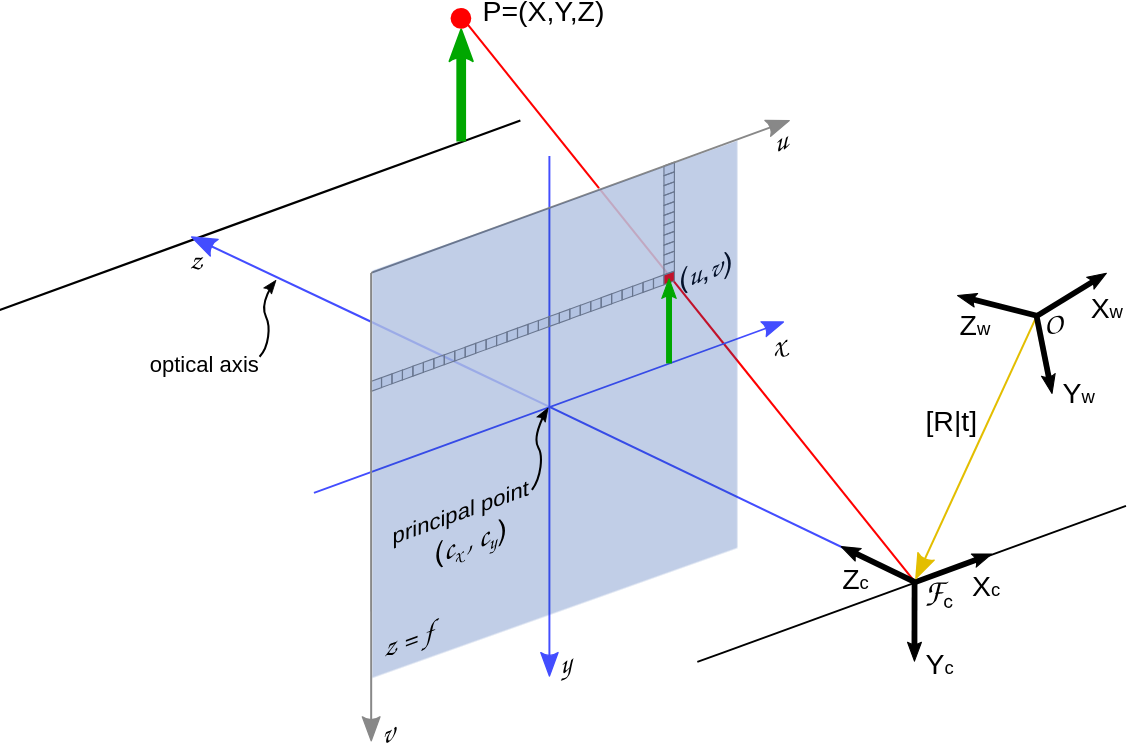
\includegraphics[width=\linewidth]{imgs/pinhole_camera.png}
\end{center}

\textbf{FoV, Sensor Width, Focal Length:} \(\displaystyle \tan\frac{\theta}{2} = \frac{W}{2f}\)

\textbf{Extrinsic Matrix:} \(\bm E_{CW} \in SE(3)\) contains the world frame to camera frame
transform. \(\bm E_{CW} = \bm E_{WC}^{-1}\) where \(\bm E_{WC}\) is the camera pose in world frame.

\textbf{Projective Matrix:} \(\tilde{\bm P} = \mattwo{\bm K}{0}{\bm 0^T}{1}\mattwo{\bm C}{\bm t}{\bm 0^T}{1} =
\tilde{\bm K}\bm E\). Project a world point to image plane as \(\tilde{\bm x}_s = \tilde{\bm P}\bar{\bm p}_w\), then
normalize by the third element.

\subsection{Distortion \& Optical Effects}

\textbf{Plumb Bob Distortion Model:} From normalized image coordinates to distorted coordinates, where
\(r = \sqrt{x_n^2 + y_n^2}\) and \(x_d, y_d\) normalized by \(f_x, f_y\):
\[
\cvec{x_d}{y_d} = (1 + \kappa _1r^2 + \kappa _2r^4 + \kappa _3r^6)\cvec{x_n}{y_n} + \cvec{2\tau _1x_ny_n + \tau _2(r^2 + 2x_n^2)}{2\tau_2 x_ny_n + \tau _1(r^2 + 2y_n^2)}
\]
Note distortion is applied after extrinsics \& projective map, but before doing intrinsics.

\textbf{Radial Distortion:} Barrel (corner points pushed in), pincushion (corner points pulled out), or mustache
(combination).

\textbf{Tangential Distortion:} Pixels shifted in one direction (further pixels shifted more), due to the lens and
imaging plane not being parallel.

\textbf{Unwarping:} Undoing distortion by precomputing distorted location of each pixel, then using bilinear
interpolation.

\textbf{Chromatic Aberration}: Differences in refraction due to wavelength cause slightly different focuses \&
magnifications (i.e. colours are misaligned).

\textbf{Vignetting:} Brightness decreases towards the edge of the image, caused by lens foreshortening, i.e. for rays
at higher angles, the size of the lens is effectively smaller, so less light comes in.

\textbf{Aliasing:} Artifacts (e.g. Moire patterns) caused by spatial sampling.

\textbf{Bayer Mosaics:} Imaging sensors have more green pixels to look natural.

\section{Image Operations \& Transformations} %%%%%%%%%%%%%%%%%%%%%%%%%%%%%%%%%%%%%%%%%%%%%%%%

\textbf{Bias/Gain (Contrast/Brightness):} \(g(i, j) = af(i, j) + b\)

\textbf{Gamma Correction:} \(g(i, j) = f(i, j)^\frac{1}{\gamma}\)

\textbf{Histogram Equalization:} \(\displaystyle T(r_k) = \sum _{j = 0}^k p_r(r_j) = \sum _{j = 0}^k \frac{n_j}{n}\)
where \(T(r_k)\) is the CDF and \(p_r(r_j)\) is the PDF (normalized histogram) as a function of pixel intensity.
Each pixel value is mapped to the proportion of pixels that it's brighter than, resulting in a flat-ish histogram.

\textbf{Linear Filtering:} \(\displaystyle g(i, j) = f * h = \sum _{k, l} f(i - k, j - l)h(k, l)\) where \(h(k, l)\)
is the \textbf{kernel}. Note how the kernel is flipped. Separable kernels can be expressed as \(\bm K = \bm v\bm h^T\)
and is equivalent to convolution by \(\bm v\) then \(\bm h\).

\textbf{Isotropic Gaussian Kernel:} Separable kernel given by
\[\displaystyle G(x, y; \sigma) = \frac{1}{2\pi\sigma^2}e^{-\frac{x^2 + y^2}{2\sigma^2}}\]

\textbf{Laplacian of Gaussian:}
\[\displaystyle \nabla^2 G(x, y; \sigma) = \left(\frac{x^2 + y^2 + 2\sigma^2}{\sigma^4}\right)G(x, y; \sigma)\]
A band-pass filter, can be used for edge/blob detection. Kernel shape like an upside down sombrero (ring of positive
values, high negative value in the centre.)

\textbf{Integral Image:} Sum of pixels up to \((i, j)\), can be computed in linear time and used to compute box filters
in linear time.
\[\alignedeqntwo{s(i, j)}{\sum _{k = 0}^i \sum _{l = 0}^j f(k, l)}{s(i - 1, j) + s(i, j - 1) - s(i - 1, j - 1) + f(i, j)}\]

\textbf{Nonlinear Filters:} Simplest examples include min/max (erosion/dilation) or median filter (removes shot noise).

\textbf{Bilateral Filter:} Soft-rejects pixels whose value differs too much from the centre; removes noise while
preserving edges, useful for image upscaling.
\[g(i, j) = \frac{\sum _{k, l} f(k, l)w(i, j, k, l)}{\sum _{k, l} w(i, j, k, l)}\]
\begin{gather*}
w(i, j, k, l) = d(i, j, k, l)r(i, j, k, l) \\
= \exp\left(-\frac{(i - k)^2 + (j - l)^2}{2\sigma_d^2}\right)\exp\left(-\frac{\norm{f(i, j) - f(k, l)}^2}{2\sigma_r^2}\right)
\end{gather*}

\textbf{Geometric Transform:} Applies to domain, \(g(\bm x) = f(\bm h(\bm x))\). Better to compute the inverse
transformation and map each pixel in the output to a location in the input, and bilinearly interpolate.

\textbf{Regularization:} For ill-conditioned problems. Combine smoothness penalty (penalize large gradients) with data
penalty.
\[
\varepsilon = \iint (f(x, y) - d(x, y))^2\,\dx\,\dy + \lambda \iint f_x^2(x, y) + f_y^2(x, y)\,\dx\,\dy
\]

\section{Image Features} %%%%%%%%%%%%%%%%%%%%%%%%%%%%%%%%%%%%%%%%%%%%%%%%

\subsection{Feature Identification and Description}

Features should be salient (distinctive), local, repeatable (can be found in other images) and compact.

\textbf{Weighted Summed Squared Difference:} Images \(I_0, I_1\), displacement \(\bm u\)
\[
E_{WSSD}(\bm u) = \sum _i w(\bm x_i)(I_1(\bm x_i + \bm u) - I_0(\bm x_i))^2
\]
For \(I_0 = I_1\) this is \textbf{autocorrelation} for a small \(\Delta\bm u\); high autocorrelation means the area is
distinctive. \(E_{AC}(\Delta\bm u) \approx \Delta\bm u^T\bm A\Delta\bm u\).
As convolution, \(\bm A = w * \mattwo{I_x^2}{I_xI_y}{I_xI_y}{I_y^2}\).

\textbf{Harris Corner Detector:} \(\det\bm A - \alpha\tr\bm A^2 = \lambda _0\lambda _1 - \alpha(\lambda _0 + \lambda _1)^2\).
Largest when both eigenvalues are large, indicating distinctiveness in both directions, i.e. a corner.

\textbf{SIFT:} Scale and rotation invariant, capable but slow. Construct scale space representation by repeated blurring
and downsampling. Find keypoints with Difference of Gaussians (similar to LoG). Reject keypoints using Hessians similar
to Harris. Assign each keypoint an orientation using gradients of points around the keypoint in a histogram. Assemble
final descriptor using 4x4 grid of subpatches, each subpatch having a gradient orientation histogram.

\textbf{SURF:} Like SIFT but faster. Uses box filters instead of Gaussians (can use integral images). Smaller descriptor
size (half as SIFT, 64-dimensional vector).

\textbf{FAST:} Very fast but not scale or rotation invariant. For each pixel look at the 16 pixels in a ring around it,
if there are 12 contiguous pixels that are brighter or darker than the centre it is a feature. Use non-maximum
suppression (suppress non-maximum features in an area around each maximum).

\textbf{BRISK:} Sample pairs of points in a circular pattern around the centre (Gaussian applied around each sampled
point); compare the pairs and generate one bit in the feature for each pair.

\textbf{BRIEF:} Draw points randomly (one of several distributions) around the centre, compare them similarly to BRISK
to form descriptor. Sampling pattern is decided once and used consistently across images. 512-bit features. Fast but not
scale/rotation invariant and sensitive to noise.

\textbf{ORB:} Combines FAST and BRIEF to get a fast and reliable feature. Downsample similarly to SIFT and apply FAST at
all scales to find keypoints. Compute orientation using intensity centroid. Use rotated BRIEF (rotate sampling pattern
or image subpatch) to form descriptor.

\textbf{Learning-Based Detectors:} Often use classic features to generate training data for supervised methods, or image
+ pose sequences for unsupervised methods. LIFT is one such method using 3 CNNs to detect, estimate orientation, and
generate descriptor, trained using contrastive learning.

\subsection{Feature Matching}

For features without descriptor, use \textbf{sum-of-squared-differences} in a local patch as distance function.
Vector-based descriptors can use \textbf{Euclidean distance}. Binary descriptors can use \textbf{Hamming distance}
(number of differing bits). Use RANSAC to reject outliers.

\subsection{Quantifying Matching Performance}

\textbf{Confusion Matrix:} To quantify matching performance. Table with true positives, false positives, false
negatives, true negatives.

\textbf{Recall/True Positive Rate:} \(TPR = TP / (TP + FN)\)

\textbf{False Positive Rate:} \(FPR = FP / (FP + TN)\)

\textbf{Precision/Positive Predictive Value:} \(PPV = TP / (TP + FP)\)

\textbf{Accuracy:} \(ACC = (TP + TN) / (TP + FN + TN + FP)\)

\vspace{-1em}
\begin{center}
    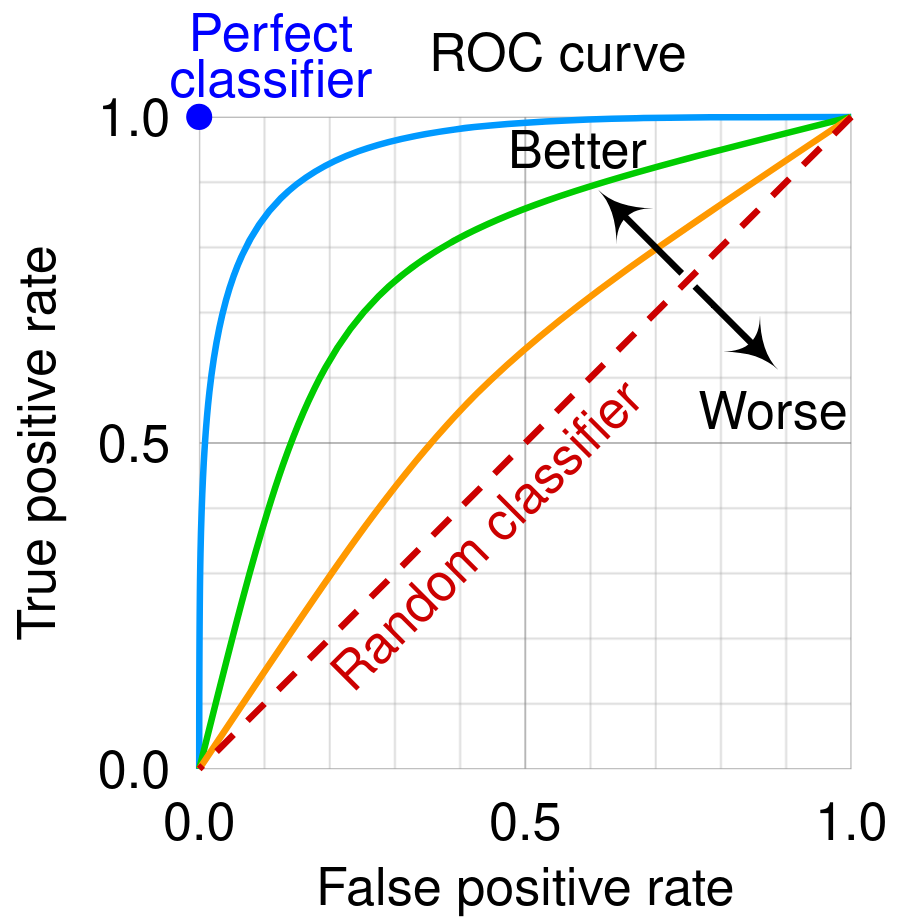
\includegraphics[width=0.5\linewidth]{imgs/roc.png}
\end{center}
\vspace{-1em}

\textbf{Receiver Operating Characteristic:} Plotting TP against FP for different values of thresholds.

\textbf{Average Precision (AP):} Area under the ROC curve.

\textbf{k-D Tree:} Multi-dimensional binary tree allowing for quick nearest neighbour queries. Built in \(O(kn\log n)\)
with \(O(n)\) space and nearest neighbours in \(O(\log n)\) time. When building, split along the median of the current
dimension at each level and cycle through dimensions until there is at most 1 data point in each partition.
For nearest neighbours:
\begin{enumerate}
    \item Find the node in the same partition as the query point by searching down the tree, and set the current min
          distance.
	\item Go back up the tree and check the following, until the root node:
    \begin{enumerate}
        \item Check the node against the current best and update if necessary.
        \item Check if the other branch can possibly contain a point closer to the query point than the current best,
              using the distance between the query point and the partitioning point, along the partitioning axis; if the
              current best is less than this, eliminate the subtree, otherwise recurse down the subtree.
    \end{enumerate}
\end{enumerate}

\textbf{Kanade-Lucas-Tomasi (KLT) Tracker:} Predict camera motion to narrow search space and match within a small area using
gradient information. Feature selection is similar to Harris. In every frame, add new features, and discard features
that have grown too dissimilar to when they were first added (based on RMS residual).

\section{Camera and Object Pose Estimation} %%%%%%%%%%%%%%%%%%%%%%%%%%%%%%%%%%%%%%%%%%%%%%%%

\textbf{Perspective-n-Point Problem:} Given 3D points and where they project to in 2D, estimate intrinsic and extrinsic
parameters.

\textbf{Direct Linear Transform (DLT):} Directly estimating entries of the projection matrix \(\bm P\); each point gives
2 equations
\begin{gather*}
x_i = \frac{p_{00}X_i + p_{01}Y_i + p_{02}Z_i + p_{03}}{p_{20}X_i + p_{21}Y_i + p_{22}Z_i + p_{23}} 
\\
y_i = \frac{p_{10}X_i + p_{11}Y_i + p_{12}Z_i + p_{13}}{p_{20}X_i + p_{21}Y_i + p_{22}Z_i + p_{23}}
\end{gather*}
Then recover \(\bm K\) and \(\bm E\) by QR factorization into upper-triangular \(\bm K = \bm R\) and orthogonal \(\bm
Q\). This is an approximate solution since often the resulting matrices are not valid (particularly rotation) due to
lack of constraints.

\textbf{Iterative Solution:} Minimize projection error \(\bm e_i = \bm x_i - f(\bm p_i; \bm C, \bm t, \bm K)\) using
nonlinear least squares (special attention to \(\bm C\) constraints).

\textbf{Wahba Problem:} Find $\bm C$ between two frames given $\bm u_i, \bm v_i$ in the frames.
\(\bm e = \bm C\bm u_i - \bm v_i\).

Using Euler angles, \(\bm J_{e_i} = \pdiff{\bm C\bm u_i}{\bm\theta}\). Each column:
\begin{gather*}
    \pdiff{\bm C\bm u_i}{\theta _3} = \skewsym{\bm 1_3}\bm C_3(\theta _3)\bm C_2(\theta _2)\bm C_1(\theta _1)\bm u_i \\
    \pdiff{\bm C\bm u_i}{\theta _2} = \bm C_3(\theta _3)\skewsym{\bm 1_2}\bm C_2(\theta _2)\bm C_1(\theta _1)\bm u_i \\
    \pdiff{\bm C\bm u_i}{\theta _1} = \bm C_3(\theta _3)\bm C_2(\theta _2)\skewsym{\bm 1_1}\bm C_1(\theta _1)\bm u_i
\end{gather*}
This breaks down at gimbal lock since Jacobian becomes zero.

Using axis-angle/matrix, \(\bm J_{e_i} = -\skewsym{\bm C_{op}\bm u_i}\).
For small rotations \(\bm C(\delta\bm\phi) \approx 1 + \skewsym{\delta\bm\phi}\).
Update operating point as \(\bm C_{op} \gets \bm C(\delta\bm\phi^*)\bm C_{op}\).

\section{Stereo Vision} %%%%%%%%%%%%%%%%%%%%%%%%%%%%%%%%%%%%%%%%%%%%%%%%

\subsection{Stereo Geometry}

\begin{center}
    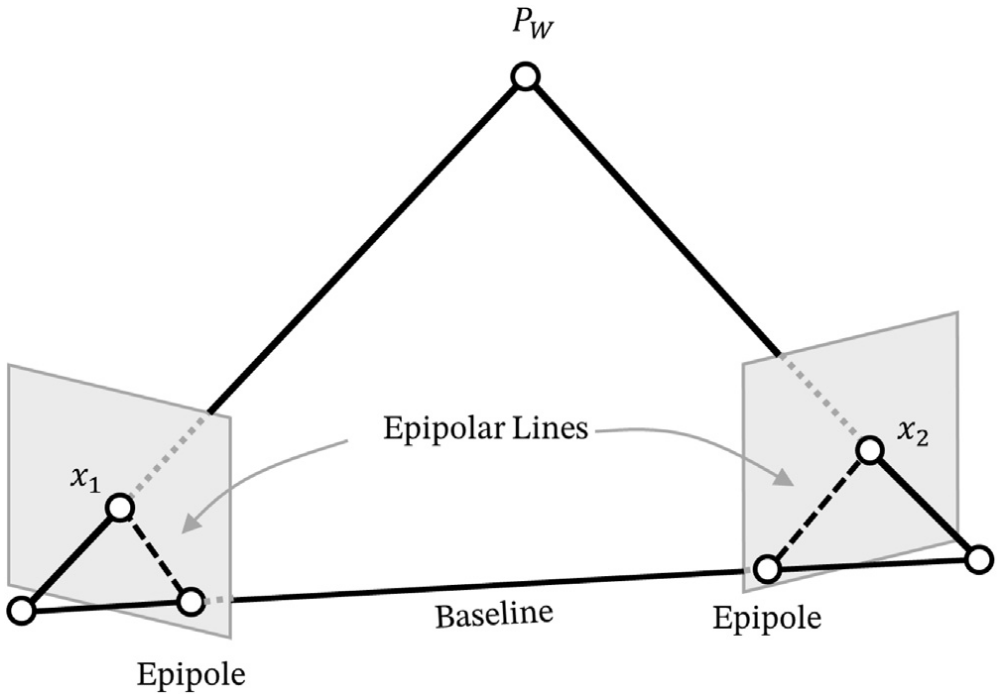
\includegraphics[width=0.8\linewidth]{imgs/epipolar.png}
    \vspace{-5mm}
\end{center}

\textbf{Epipolar Geometry:} Form the epipolar plane from a point and the cameras' optical centres; the intersection
of the epipolar plane with each imaging plane forms an epipolar line, which is where correspondences lie.

\textbf{Stereo Rectification:} Transforming and unwarping the images so the imaging planes become parallel, at the same
depth, and rotationally aligned (fronto-parallel or standard rectified geometry). After rectification all epipolar lines
are horizontal.

\textbf{Disparity:} Difference in \(x\) values of a point between cameras. \(Z = \frac{fb}{d}\) where \(b\) is baseline
and \(d\) is disparity. Larger disparity indicates a point is closer.

\textbf{Stereo Camera Model:}
\(\displaystyle\cvec{x_0}{y_0}{d} = \bm f(\bm p_c) = \frac{f}{Z}\cvec{X}{Y}{b} + \cvec{c_x}{c_y}{0}\)

\textbf{Baseline:} Distance between cameras. Larger baseline improves accuracy, but makes matching more difficult as
overlapping FOV decreases and foreshortening is increased (oblique objects appear as different sizes). Wider baseline
also makes errors more Gaussian-like (shorter tail); for short baseline, using Gaussian errors biases the points to be
closer.

\subsection{Stereo Matching}

\textbf{Local Methods:} Sliding a small window along the epipolar line, without using global info. Computes similarity
within window, e.g. sum-of-squared/absolute-differences, or normalized cross-correlation or gradient based. Larger
window sizes result in smoother and less noisy images but loses detail.

\textbf{Learning-Based Methods:} Often using CNNs to combine local and global aggregation. Produces smoother depth maps.
Often trained on synthetic datasets.

\subsection{Invertible Stereo Models}

\textbf{Combined Stereo Model:} Forward model produces pixel locations in both cameras. Frame origin is halfway between
two cameras.

\begingroup
\thinmuskip=3mu       % Readable sin/cos
\medmuskip=2mu        % Tight + and -
\thickmuskip=3mu      % Tight =
Forward: \(\displaystyle f(\bm p) = \bm M\frac{1}{z}\bm p = \matfour{f_u}{0}{c_u}{f_u\frac{b}{2}}{0}{f_v}{c_v}{0}{f_u}{0}{c_u}{-f_u\frac{b}{2}}{0}{f_v}{c_v}{0}\frac{1}{z}\bm p = \cvec{u_l}{v_l}{u_r}{v_r}\). \\
\endgroup
Inverse model: \(\displaystyle \bm g(\bm y) = {\displaystyle\frac{b}{u_l - u_r}}\cvec{\frac{1}{2}(u_l + u_r) - c_u}{\frac{f_u}{f_v}\left(\frac{1}{2}(v_l + v_r) - c_v\right)}{f_u}\). \\
\mbox{Jacobians: forward \(\displaystyle\pdiff{\bm f}{\bm p} = \bm M\frac{1}{p_3}\matfour{1}{0}{-{p_1}/{p_3}}{0}{0}{1}{-{p_2}/{p_3}}{0}{0}{0}{0}{0}{0}{0}{-{p_4}/{p_3}}{1}\),
inverse \(\displaystyle\pdiff{\bm g}{\bm y} =\)}\\ % FUCK LATEX
\begingroup
\setlength{\arraycolsep}{2pt} 
\[\frac{b}{(u_l - u_r)^2}\mat{\mrow{-u_r + c_u}{0}{u_l - c_u}{0}\mrow{-\frac{f_u}{f_v}\left(\frac{1}{2}(v_l + v_r) - c_v\right)}{\frac{f_u}{2f_v}}{\frac{f_u}{f_v}\left(\frac{1}{2}(v_l + v_r) - c_v\right)}{\frac{f_u}{2f_v}}\mrow{-f_u}{0}{f_u}{0}}\]
\endgroup

\textbf{Pixel-Disparity Stereo Model:} Forward model produces a pixel location and disparity. Frame origin is at the
left camera.

\begingroup
\thinmuskip=3mu       % Readable sin/cos
\medmuskip=2mu        % Tight + and -
\thickmuskip=3mu      % Tight =
Forward: \(\displaystyle \bm y = \bm f(\bm p) = \bm M\frac{1}{p_3}\bm p = \mat{\mrow{f_u}{0}{c_u}{0}\mrow{0}{f_v}{c_v}{0}\mrow{0}{0}{0}{f_ub}}\frac{1}{p_3}\bm p = \cvec{u_l}{v_l}{d}\). \\
\endgroup
Inverse model: \(\displaystyle \bm g(\bm y) = \frac{b}{d}\cvec{u_l - c_u}{\frac{f_u}{f_v}(v_l - c_v)}{f_u}\).

Forward Jacobian: \(\displaystyle \pdiff{\bm f}{\bm p} = \frac{1}{p_3}\bm M\matfour{1}{0}{-p_1/p_3}{0}{0}{1}{-p_2/p_3}{0}{0}{0}{0}{0}{0}{0}{-p_4/p_3}{1}\) \\
Inverse Jacobian: \(\displaystyle \pdiff{\bm g}{\bm y} = \frac{b}{d^2}\matthree{d}{0}{c_u - u_l}{0}{\frac{f_u}{f_v}d}{\frac{f_u}{f_v}(c_v - v_l)}{0}{0}{-f_u}\)

\section{Camera Calibration} %%%%%%%%%%%%%%%%%%%%%%%%%%%%%%%%%%%%%%%%%%%%%%%%

\textbf{Calibration:} Characterizing camera properties, including geometric (determining distortion and \(\bm K\); most
common) or photometric (determining optical effects and getting consistent brightnesses; harder and less common).

For geometric, given image coordinates \(\bm x_{ij}\) for point \(i\) in observed from pose \(j\) and target points
\(\bm p_i\), recover all parameters in \(\bm x_{ij} = f(\bm p_i; \bm C_j, \bm t_j, \bm K, \bm\kappa, \bm\tau)\).

\textbf{Calibration Targets:} Most commonly checkerboard (N-planes approach) due to ease of detection, precision of
corners, and invariance to foreshortening.

\textbf{Solution:} Use nonlinear least squares (DLT has no distortion and fails for coplanar points). Parameter
\(\theta\) contains calibration parameters and all poses. Minimize reprojection error:
\begingroup
\thinmuskip=3mu       % Readable sin/cos
\medmuskip=2mu        % Tight + and -
\thickmuskip=3mu      % Tight =
\[E(\delta\bm\theta) = \sum _{ij}\norm*{\pdiff{f}{\bm C_j}\delta\bm C_j + \pdiff{f}{\bm t_j}\delta\bm t_j + \pdiff{f}{\bm K}\delta\bm K + \pdiff{f}{\bm\kappa}\delta\bm\kappa + \pdiff{f}{\bm\tau}\delta\bm\tau - \bm r_{ij}}^2\]
\endgroup

\textbf{Stereo Calibration:} Additionally solve for \(\bm T_{R,L}\), the rigid transform from left camera to right
camera. \(\tilde{\bm P}_L = \tilde{\bm K}\bm T_{L,W}, \tilde{\bm P}_R = \tilde{\bm K}\bm T_{R, L}\bm T_{L,W}\).
Parameter vector has both camera calibration parameters, left camera pose for each image, and transform between cameras.

\textbf{Jacobian Structure:} Sparse, only the extrinsics for pose \(j\) affects \(\bm x_{ij}\), but \(\bm K, \bm\kappa,
\bm\tau\) affects all measurements made with that camera. Can be exploited using sparse Cholesky factorization.

\begin{center}
    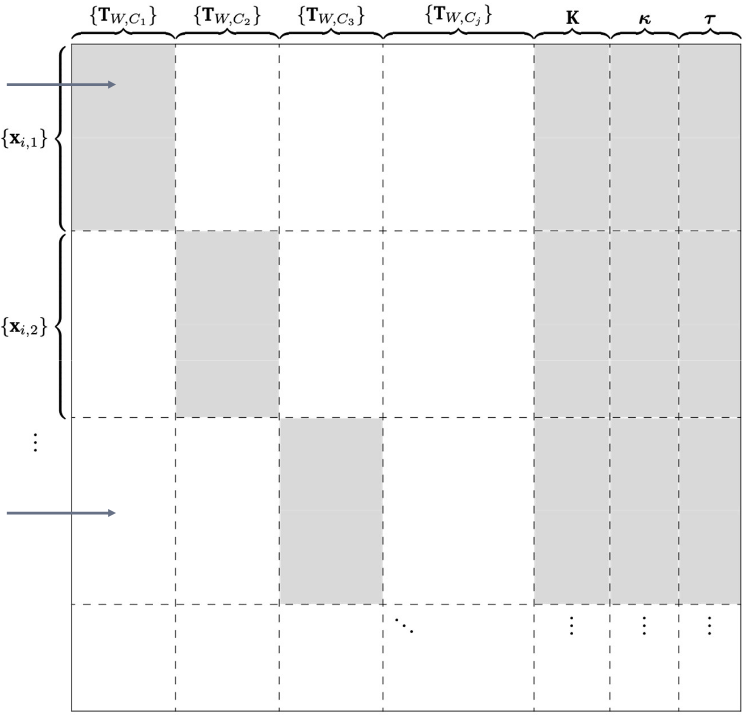
\includegraphics[width=0.45\linewidth]{imgs/calib_jacobian_structure.png}
    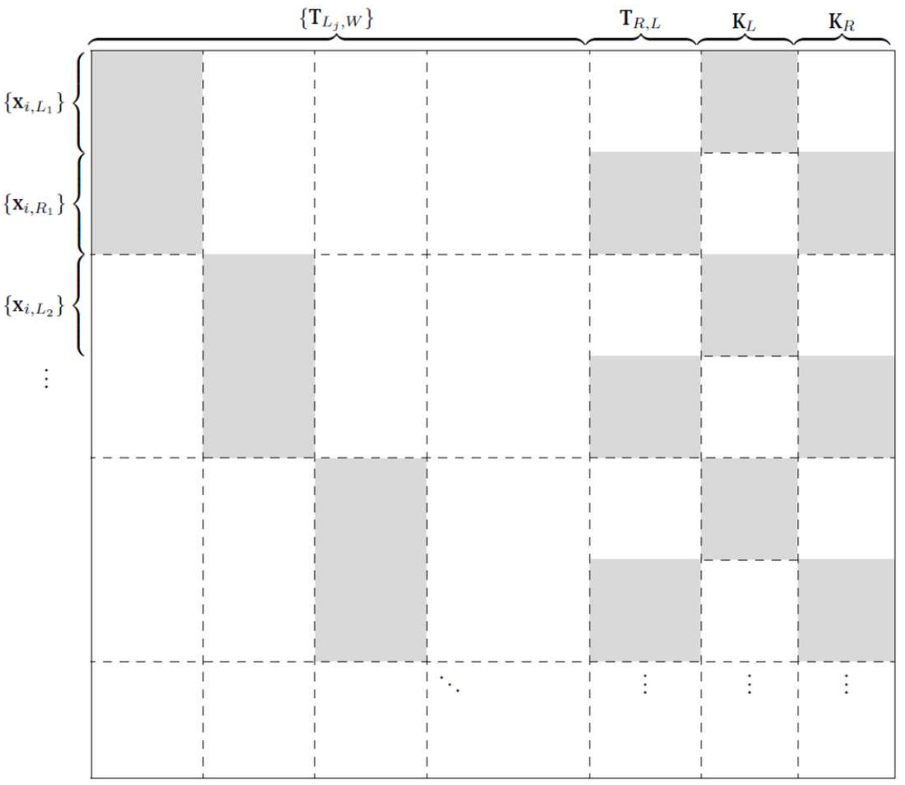
\includegraphics[width=0.51\linewidth]{imgs/calib_stereo_jacobian_structure.png}
\end{center}

\section{Sparse SfM, Visual Odometry, and SLAM} %%%%%%%%%%%%%%%%%%%%%%%%%%%%%%%%%%%%%%%%%%%%%%%%

\subsection{Structure from Motion}

\textbf{Structure from Motion:} Determining 3D positions of landmark points (structure) and camera poses (motion) from
image feature correspondences. Can be solved up to scale if camera poses are unknown.

\vspace{-1em}
\begin{center}
    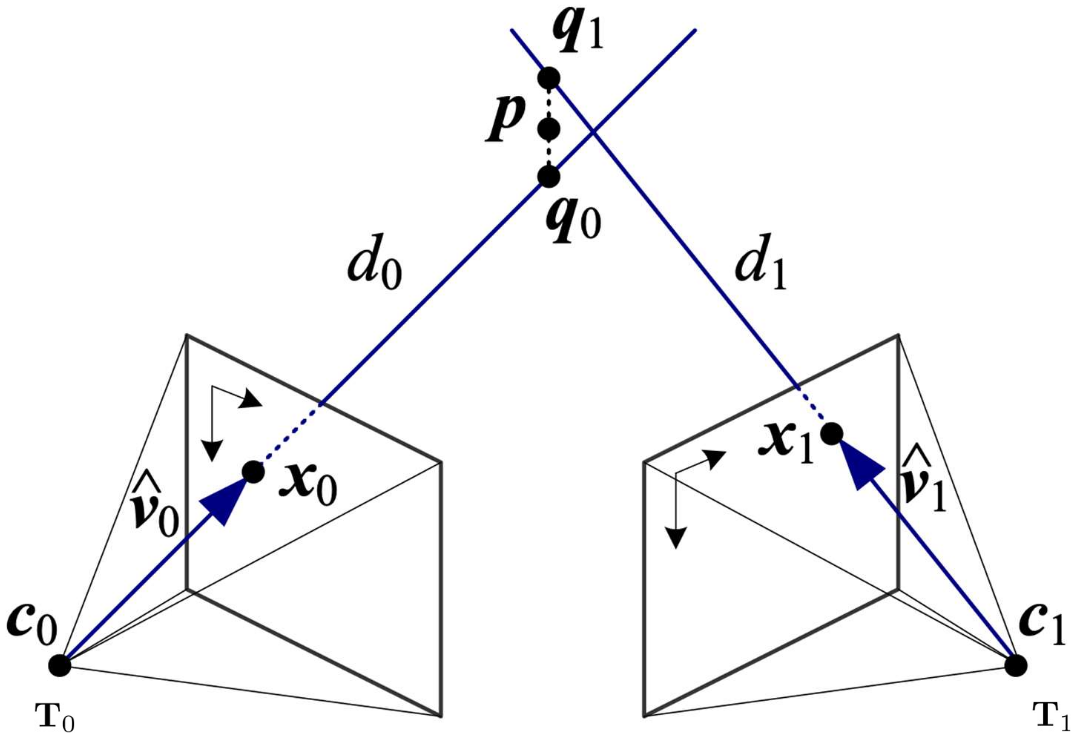
\includegraphics[width=0.6\linewidth]{imgs/triangulation.png}
\end{center}
\vspace{-1em}

\textbf{Triangulation:} Given $\bm x_j, \bm K_j$ and pose \(\bm C_j, \bm c_j\) for each camera, find the point $\bm p$
closest to all of the rays from each camera. Each ray has unnormalized direction \(\bm v_j = \bm C_j^{-1}\bm
K_j^{-1}\bar{\bm x}_j\). Optimal distance \(d_j = \hat{\bm v}_j \cdot (\bm p - \bm c_j)\) minimizes error \(\norm{\bm
c_j + d_j\hat{\bm v}_j - \bm p}^2\), results in optimal point \(\bm q_j = \bm c_j + (\hat{\bm v}_j\hat{\bm v}_j^T)(\bm p
- \bm c_j)\). Least squares to minimize distance between \(\bm p\) and each \(\bm q_j\).

\textbf{Bundle Adjustment:} Using NLS to jointly optimize the 3D structure (through triangulation) and camera poses (and
possibly calibration).

\textbf{Optimizations:} Naive NLS is cubic in number of parameters. Exploit sparse Jacobian and Hessian (\(\bm J^T\bm
J)\) structure. Order parameters by grouping relevant parameters and putting global parameters last. Use sliding windows
to optimize a fixed horizon or select keyframes to optimize fewer frames for very large problems (SLAM). Use Kalman
filters for incremental solutions.

\textbf{Parametrizations:} Should be close to linear so NLS is locally quadratic. Use homogeneous coordinates
\(\tilde{\bm x} = (\tilde x, \tilde y, \tilde z, \tilde w)\) for landmark points to handle points at infinity. For
rotations use quaternions or matrices.

\textbf{Jacobian/Hessian Structure:} Jacobian has a row for each observation (each feature in each camera), a column for
each unique feature's 3D location, and one for each camera's parameters. Dense block between observation and feature
when the feature appears in that observation, between observation and camera when the observation comes from that camera.
Hessians are somewhat diagonal since 3D feature locations don't affect each other.

\textbf{Robust Estimators:} Solution is sensitive to outliers, so in addition to RANSAC, cost of outliers should be
downweighted. Instead of L2, use M-estimators or cost functions that become linear or flatten out for large errors to
weigh outliers less. Might reduce region of convergence.

\begin{center}
    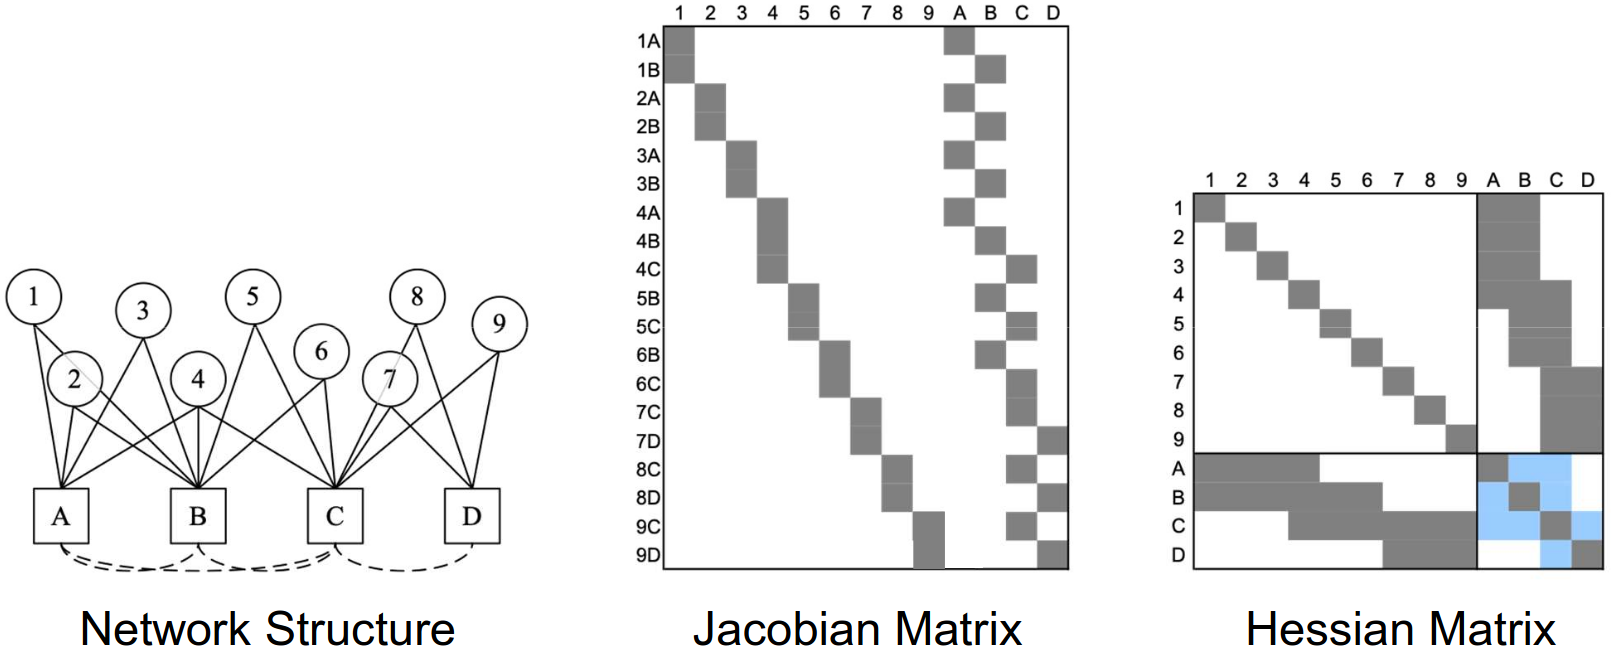
\includegraphics[width=\linewidth]{imgs/ba_jacobian_structure.png}
    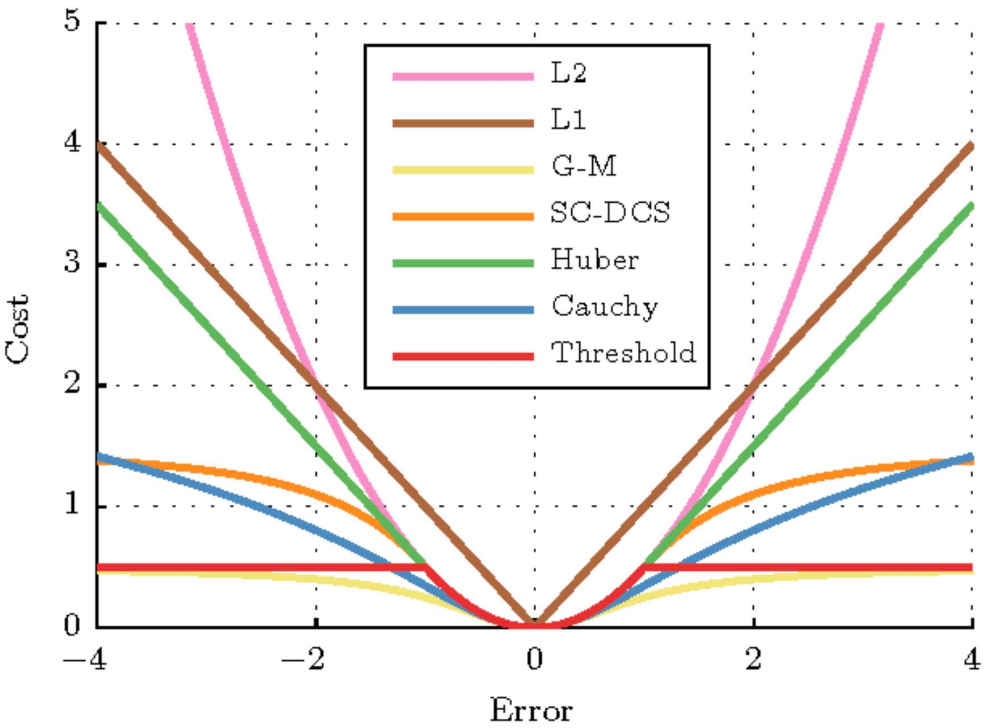
\includegraphics[width=0.7\linewidth]{imgs/losses.png}
\end{center}


\subsection{Incremental SfM/Visual Odometry}

\textbf{Visual Odometry:} Given images captured in frame \(a\) and frame \(b\), find \(\bm T_{ba}\). Use where high
accuracy short-term localization is needed and no external options, e.g. indoors, Mars, or high wheel slip environments.

\textbf{Taxonomy:} \textit{Monocular} (non-invertible observation model) vs. \textit{stereo} (invertible);
\textit{feature-based/sparse} (extract \& match features) vs. \textit{intensity-based} (directly match image intensities).

\textbf{VO Pipeline:} Stereo dewarp and rectify, detect features and stereo match, match features with previous frame,
outlier rejection, finally solve for pose transform with NLS, potentially with other sensors.

\textbf{Point Cloud Alignment:} Given \(\bm p_a^j, \bm p_b^j\), minimize cost
\[E(\bm C_{ba}, \bm r_a) = \frac{1}{2}\sum _{j = 1}^J \left(\bm p_b^j - \bm C_{ba}(\bm p_a^j - \bm r_a)\right)^T\bm\Sigma^j\left(\bm p_b^j - \bm C_{ba}(\bm p_a^j - \bm r_a)\right)\]
with matrix weights \(\bm\Sigma^j = \left(\bm G_b^j\bm R_b^j{\bm G_b^j}^T + \bm C_{ba}\bm G_a^j\bm R_a^j{\bm G_a^j}^T\bm C_{ba}^T\right)^{-1}\)
where \(\bm G_b^j = \eval{\pdiff{\bm g}{\bm y}}{\bm f(\bm p_b^j)}, \bm G_a^j = \eval{\pdiff{\bm g}{\bm y}}{\bm f(\bm p_a^j)}\), and $\bm R_b^j, \bm R_a^j$ are pixel measurement covariances.
Closed-form solution for scalar weights:
\begin{enumerate}
	\item Align centroids: $\displaystyle\bm p_a = \frac{\sum _{j = 1}^J w^j\bm p_a^j}{\sum _{j = 1}^J w^j}, \bm p_b = \frac{\sum _{j = 1}^J w^j\bm p_b^j}{\sum _{j = 1}^J w^j}$
	\item Outer product: $\displaystyle\bm W_{ba} = \frac{1}{\sum _{j - 1}^J w^j}\sum _{j = 1}^J w^j(\bm p_b^j - \bm p_b)(\bm p_a^j - \bm p_a)^T$
	\item Compute SVD $\bm V\bm S\bm U^T = \bm W_{ba}$, then compute rotation \(\bm C_{ba} = \bm V\matthree[bsmall]{1}{0}{0}{0}{1}{0}{0}{0}{\det(\bm U)\det(\bm V)}\bm U^T\),
          and translation \(\bm r_a = -\bm C_{ba}^T\bm p_b + \bm p_a\).
\end{enumerate}

\section{Optical Flow} %%%%%%%%%%%%%%%%%%%%%%%%%%%%%%%%%%%%%%%%%%%%%%%%

\textbf{Optical Flow:} Estimating a motion vector for every pixel in the image from a series of images, resulting in an
optical flow field. Ill-posed problem due to the aperture problem.

\textbf{Brightness Constancy Assumption:} \[I(x, y, t) = I(x + \Delta x, y + \Delta y, t + \Delta t)\]
i.e. the corresponding pixel in the next image has the same brightness, where \((\Delta x, \Delta y)\) is the flow vector we want.

\textbf{Flow Equation:} \[\pdiff{I}{x}v_x + \pdiff{I}{y}v_y + \pdiff{I}{t} = 0 \iff I_xv_x + I_yv_y = \Delta I^T\bm v = -I_t\]
obtained from Taylor expansion of brightness constancy.

\textbf{Lucas-Kanade Method:} Assuming each small patch has the same flow and uses only local information.
Matrix equation for each patch:
\[\matthreetwo{I_x(\bm p_1)}{I_y(\bm p_1)}{\vdots}{\vdots}{I_x(\bm p_N)}{I_y(\bm p_N)}\cvec{u}{v} = -\cvec{I_t(\bm p_1)}{\vdots}{I_t(\bm p_N)} \iff \bm A\bm d = \bm b\]
\[\mattwo{\sum I_xI_x}{\sum I_xI_y}{\sum I_xI_y}{\sum I_yI_y}\cvec{u}{v} = -\cvec{\sum I_xI_t}{\sum I_yI_t} \iff (\bm A^T\bm A)\bm d = \bm A^T\bm b\]

\textbf{Horn-Schunck Method:} Uses a smoothness regularization term, so large changes in flow vector between adjacent
pixels is penalized:
\[E = \iint [(I_xu + I_yv + I_t)^2 + \alpha^2(\norm{\Delta u}^2 + \norm{\Delta v}^2)]\,\dx\,\dy\]
where \(\alpha\) is the regularization constant and \(\Delta u, \Delta v\) are flow vector gradients.
Practically we take the derivative and convert to summation, then use NLS to solve.
Can help fill in textureless regions, at the cost of blurring boundaries.

\textbf{Control Applications:} Objects further away move slower, so we can get relative depth info. A simple navigation
rule is to steer so that optical flows of 2 cameras on two sides are equal, to centre the robot between two walls.

\section{Dense/Photometric Mapping} %%%%%%%%%%%%%%%%%%%%%%%%%%%%%%%%%%%%%%%%%%%%%%%%

\textbf{Dense Mapping:} Match images and produce a pose between frames based on image intensities only, without
extracting features, and using (almost) every pixel to construct the map, i.e. solving pixel correspondence and camera
pose estimation at once, instead of decoupling them like in sparse VO.

\textbf{Comparison to Sparse Mapping/VO:}
\begin{enumerate}
    \item More robust to common failure modes due to inclusion of global information, e.g. blur, self-similar textures, defocus
    \item Uses almost all information in the image (as opposed to only pixels around features)
    \item Dense maps enable scene understanding and path planning
    \item Implicit data association by matching pixel intensities
    \item Very high dimensionality ($10^5$ to $10^6$ pixels per image), computationally expensive
    \item Contains a lot more local minima (due to implicit data association), sensitive to initialization (works only for small camera movements)
\end{enumerate}

\textbf{Dense Map Representations:} Surface-based: meshes, splines (fitting splines to points), height/depth maps;
Point-based: point clouds, surfels (like voxels but for a small 2D surface patch), Gaussian splats (blob with centre,
covariance and colour); Volume-based: voxel grids (e.g. octrees for adaptive resolution), signed distance functions.

\begin{center}
    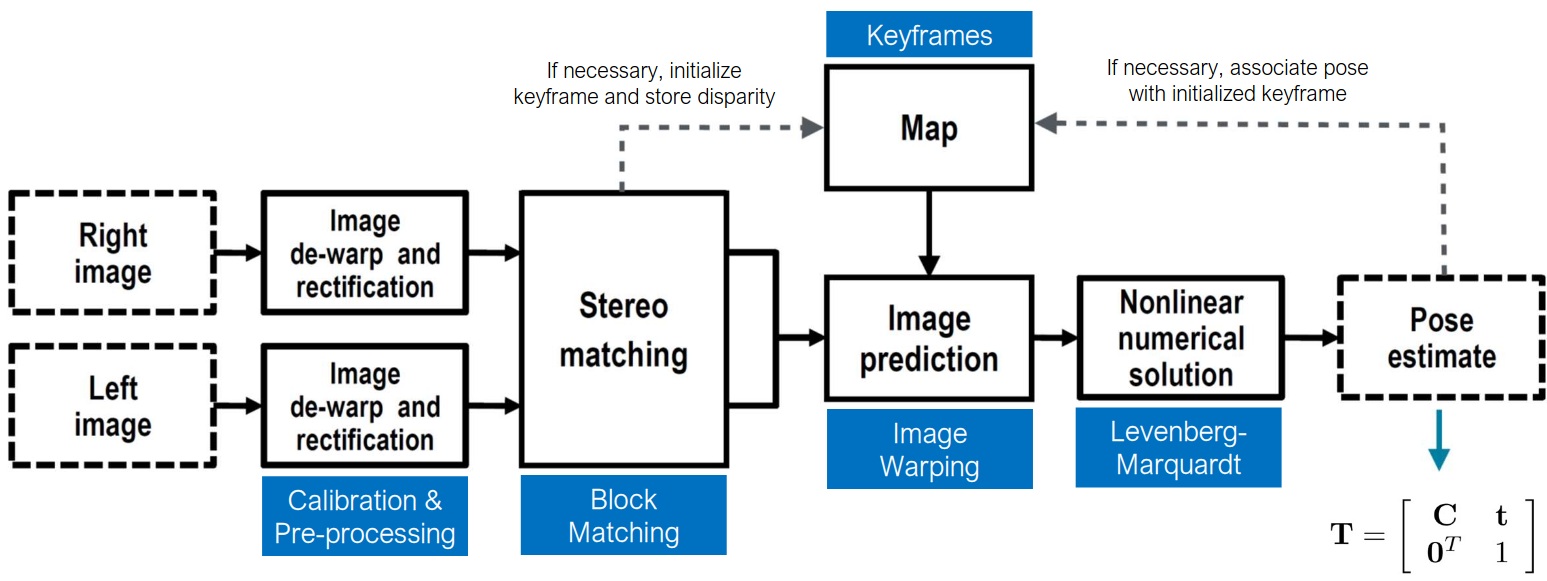
\includegraphics[width=\linewidth]{imgs/dense_mapping_pipeline.png}
\end{center}

\textbf{Image Warping:} Given the location of a pixel in frame \(k - 1\) and pose transformation \(\bm T_{k, k - 1}\),
\(\cvec{u_k}{v_k}{d_k} = \bm f\left(\bm T_{k, k - 1}\bm g\left(\cvec{u_{k - 1}}{v_{k - 1}}{d_{k - 1}}\right)\right)\).

\textbf{Photometric Error:} \(e_i = I_{k - 1}(\bm u_{k - 1}^i) - I_k'(\bm u_k^i)\) where \(I_k'\) is interpolated from
\(I_k\), indexed with continuous coordinates \(\bm u_k^i\), and
\(\bm y_k^i = \cvec{\bm u_k^i}{d_k^i} = \bm f(\bm T_{k, k - 1}\bm g(\bm y_{k - 1}^i))\) from image warping.
Solve for optimal pose transform \(\displaystyle \hat{\bm T}_{k, k - 1} = \argmin _{\bm T_{k, k - 1}}\sum _{i = 1}^N\left(\frac{1}{\sigma}e_i\right)^2\).

\textbf{Disparity-Included Error:} \(\displaystyle \bm e_i = \cvec{I_{k - 1}(\bm u_{k - 1}^i) - I_k'(\bm u_k^i)}{d_k^i -
\bar D_k'(\bm u_k^i)}{d_{k - 1}^i - \bar d_{k - 1}^i}\) \\ to optimize keyframe disparity for better mapping. $d_{k - 1}$
is the disparity to be optimized, $\bar d_{k - 1}$ is the observed disparity
(from stereo matching) in the previous frame, and $\bar D_k'$ is the interpolated observed disparity in the current frame.
Use matrix weights for optimization.

\textbf{Coarse-to-Fine Optimization:} Starting with a blurred and subsampled image, then repeatedly optimizing while
increasing resolution, using the previous optimization result as the initial guess for the next iteration. First
iteration can use IMU/odometry. This smoothes out local minima and increases region of convergence.

\textbf{Selective Pixel Matching:} Performing matching/optimization only over "informative" pixels, based on gradient
magnitude. Divide image into a grid, and for each cell take only the pixel with the largest gradient magnitude for
optimization.

\textbf{Apply Photometric Calibration:} Dense mapping is affected by gamma, exposure, vignetting, etc., so photometric
calibration can be used to build a model correcting these effects.

\section{Classical Image Segmentation} %%%%%%%%%%%%%%%%%%%%%%%%%%%%%%%%%%%%%%%%%%%%%%%%

\textbf{Segmentation Types:} \textit{Coarse} (bounding boxes for objects) vs. \textit{fine} (splines or pixel-wise
masks/labels to describe boundaries between objects). \textit{Semantic}: segmenting based on object types;
\textit{instance}: segmenting based on object types and different instances of the same type; \textit{panoptic}:
segmenting instances of countable foreground objects, and regions of uncountable background "stuff".

\textbf{Thresholding:} Simplest method; applying a threshold to image intensity values (or to specific channels in some
colour space), then finding connected components.

\textbf{Active Contours:} An energy-minimization approach to fit a spline \(\bm f(s) = (u(s), v(s))\) to minimize the
energy consisting of the smoothness cost 
\(\mathcal E_\text{int} = \int \alpha(s)\norm{\bm f_s(s)}^2 + \beta(s)\norm{\bm f_{ss}(s)}^2\,\ds\)
and image energy \(\mathcal E_\text{image} = w_\text{line}\mathcal E_\text{line} + w_\text{edge}\mathcal E_\text{edge} + w_\text{term}\mathcal E_\text{term}\)
where \(\mathcal E_\text{edge} = \sum _i -\norm{\nabla I(\bm f(i))}^2\).
The terms attract the spline to dark ridges, strong gradients, and line terminations respectively.

\textbf{B-Splines:} \(\bm f(s) = \sum _k B_k(s)\bm x_k\), where $B_k(s)$ are $k$ basis functions and $\bm x_k$ are
control points (i.e. parameters); generalizations of Bezier curves.

\textbf{Dynamic contours:} Model evolving contours with discrete linear dynamics: $ \bm{x}_t = \bm{A} \bm{x}_{t-1}
+\bm{w}_t$. Account for multi-modal uncertainty with particle filtering. Known as Conditional Density
Propagation/CONDENSATION.

\textbf{Split-and-Merge/Watershed:} Starting from seed points, perform watershed segmentation: Interpret the image
intensities as "heights" and fill the local minima with "water", i.e. propagate outward from the minima until we hit a
high-intensity boundary. Assumes that the boundaries are similar in intensity. Locality constraints can be applied to
close off the regions.

\textbf{Mean-Shift Algorithm:} Cluster pixels in colour space (e.g. LUV) by considering each pixel as a sample from a
probability distribution with multiple means, using kernel density estimation to find the PDF, where each mode is a
segment.
\begin{enumerate}
    \item For each mode $\bm y$, start with some initial guess $\bm y_0$.
    \item $\displaystyle\bm y_{k + 1} = \bm y_k + \bm m(\bm y_k) = \frac{\sum _i\bm x_iG(\bm y_k - \bm x_i)}{\sum _i G(\bm y_k - \bm x_i)}$ where $\bm m(\bm y_k)$ is the mean-shift, $G$ is the derivative of the kernel density estimator.
    \item Repeat until convergence, $\norm{\bm m(\bm y_k)} < \epsilon$.
\end{enumerate}
Initialize a mode at each input point, and iterate until all pixels have converged to a mode; then each distinct mode
will be a segment.

\textbf{Kernel Density Estimator:} $\displaystyle f(\bm x) = \sum _i k\left(\frac{\norm{\bm x - \bm x_i}^2}{h^2}\right)$
for samples $\bm x_i$, mean $\bm x$, bandwidth (spread) \(h\), and kernel function \(k(r)\).
Gaussian kernel $\displaystyle k_N(r) = \exp\left(-\frac{1}{2}r\right)$ is commonly used.

\textbf{Graph Cuts:} Construct a graph from the image and cut it into regions. Nodes are pixels. Edges are weighted
using an affinity function based on salient properties, e.g. pixel distance, intensity difference, colour difference,
texture metrics (e.g. by convolution). Can make minimum cuts (using the max-flow/min-cut algorithm, efficient but tends
to over-segment), or normalized cuts (cost of the cut normalized by the size of segments, NP-hard but can be
approximated).

\textbf{Markov Random Fields Formulation:} Segmentation label for each pixel are the "true" pixel states \(x_i\), and
the image itself is the observed "evidence" \(y_i\). Minimize energy $E(x, y) = \sum _i \varphi(x_i, y_i) + \sum
_{ij}\psi(x_i, x_j)$ where \(\varphi\) encodes the segmentation class and \(\psi\) encodes smoothness. Can be formulated
as a min-cut problem for binary (foreground/background) labelling.

\textbf{GrabCut:} Segments using a user-supplied bounding box and an MRF model. A Gaussian mixture model (GMM) is fit to
the foreground and background using the bounding box. The MRF energy is defined based on the GMM, and min-cut is applied
to classify into foreground and background. Repeat until convergence, fitting a new GMM each time with the new
foreground-background segmentation.

\section{Visual Servoing} %%%%%%%%%%%%%%%%%%%%%%%%%%%%%%%%%%%%%%%%%%%%%%%%

Controlling a robot (usually a manipulator) relative to a target of interest, by tracking visual features. The camera
can be mounted on the robot (\textbf{eye-in-hand}) or at a fixed external point. For eye-in-hand there is a risk of
moving too quickly and losing sight of the target.

\subsection{Position-Based Visual Servoing}

Using known calibration and target geometry (i.e. 3D positions of feature points) to estimate target pose, and control
the robot in task space (e.g. $SE(3)$) to move to a desired pose \(\bm T_{TE}^*\) relative to the target.

Estimate target pose by minimizing the error function $\bm e_i = \bm x_i - \bm f(\bm p_i; \bm C, \bm t, \bm K)$.
Requires depth to be estimated or approximated based on target size. Commonly done with fiducial markers like ArUco or
AprilTag, with motion estimation using Kalman filtering or particle filtering, either in an inertial frame or a frame
relative to the moving camera.

Controller can be \textit{end-point open-loop} (using inverse kinematics to move the arm directly to the desired
location, often used for external camera) or \textit{eye-in-hand closed-loop} (setting the end-effector velocity based
on pose error).

\textbf{Limitations:} No guarantee target image feats will stay in FOV. Can resolve with extra constraints, finite
horizon planing, \& numerical optimization. Assumes scale/depth knowledge from a known target. Can also solve with
approx depths or locking scale on initialization.

\subsection{Image-Based Visual Servoing}

For hand-in-eye configurations, directly tracking the image feature positions in image space, without explicitly
computing the target pose, usually using a linear controller in image space.

Use the camera model Jacobian to solve for the desired camera velocity vector, given the difference between actual \(\bm
p_i\) and desired \(\bm p_i^d\) feature points for at least 3 non-colinear points:
\begingroup
\everymath{\displaystyle}
\thinmuskip=3mu       % Readable sin/cos
\medmuskip=2mu        % Tight + and -
\thickmuskip=3mu      % Tight =
\setlength{\arraycolsep}{2pt}
\[\dot{\bm p} = \cvec{\dot u}{\dot v} = \mat{\mrow{-\frac{f}{Z}}{0}{\frac{u}{Z}}{\frac{uv}{f}}{-\frac{f^2 + u^2}{f}}{v}\mrow{0}{-\frac{f}{Z}}{\frac{v}{Z}}{\frac{f^2 + v^2}{f}}{-\frac{uv}{f}}{-u}}\cvec{v_x}{v_y}{v_z}{\omega _x}{\omega _y}{\omega _z} = \bm J_p\bm\nu\]
\[\cvec{\dot{\bm p}_1}{\vdots}{\dot{\bm p}_n} = \cvec{\bm J_{p_1}}{\vdots}{\bm J_{p_n}}\bm\nu \implies \bm\nu = \lambda\cvec{\bm J_{p_1}}{\vdots}{\bm J_{p_n}}^\dagger\cvec{\bm p_1^d - \bm p_1}{\vdots}{\bm p_n^d - \bm p^n}\]
\endgroup

\textbf{Limitations:} Since camera motion is calculated implicitly, can fail to converge for cases where movement is
ambiguous, e.g. rotation by \(\pi\) for rectangular set of feature pts. Requires feat. depth estimates but usually
robust to them.

\section{Alternative Imaging Systems} %%%%%%%%%%%%%%%%%%%%%%%%%%%%%%%%%%%%%%%%%%%%%%%%

\textbf{Event Camera:} Measures light intensity variations in a scene, asynchronously for every pixel. Instead of
outputting intensity values, an event is triggered when \(L(x, y, t + \Delta t) - L(x, y, t) = \pm C\) where \(L(x, y,
t) = \log I(x, y, t)\). Each event is a tuple \((t, x, y, \sign\diff{I}{t})\). For a point moving with velocity \(\bm u
= (u, v)\), events are generated where \(-\Delta L \cdot \bm u = \pm C\), i.e. events are triggered along edges in the
image when movement is perpendicular to an edge.

\begin{center}
    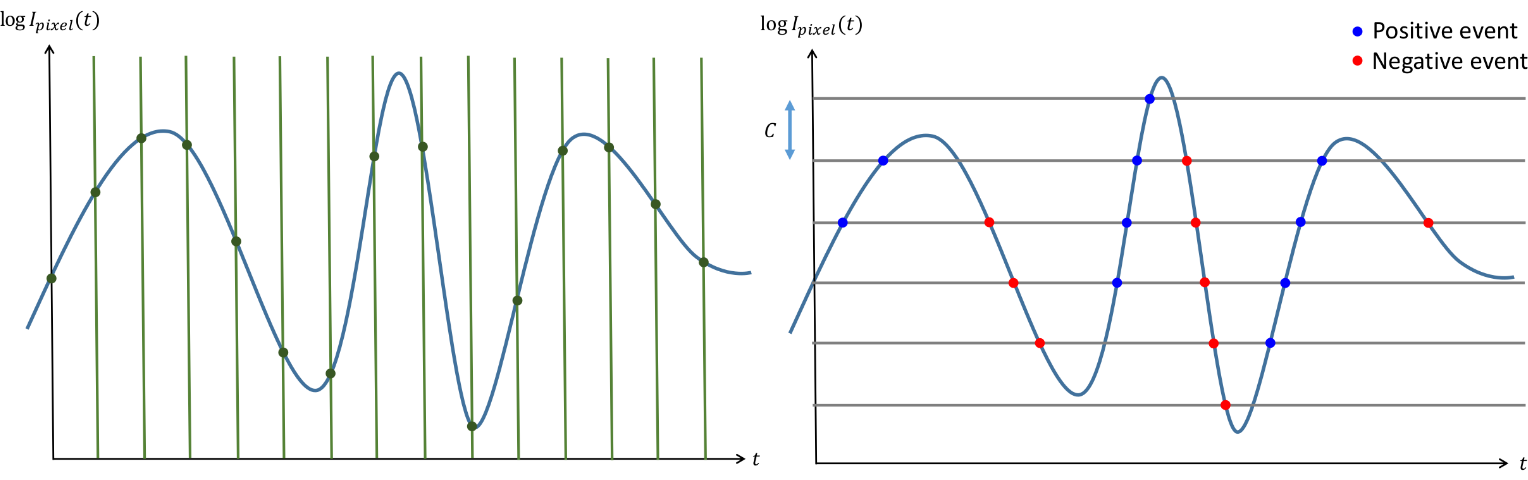
\includegraphics[width=\linewidth]{imgs/event_cam.png}
\end{center}

Advantages include much higher dynamic range (140 dB), very low latency/high framerate (1 MHz), negligible motion blur,
low bandwidth use, and very low power consumption. Applications include capturing very fast motions and removing motion
blur when combined with traditional camera.

\textbf{Thermal Camera:} Measures the infrared spectrum instead of visible light. Can see with no light since objects
emit their own infrared radiation, can see through fog, smoke, etc, and determine temperature of objects. Not
photometrically consistent over time due to the camera heating itself, non-uniform sensor responses, and spatial
artifacts, which requires calibration to remove. Can be combined with conventional cameras, especially in low-light
scenarios where thermal cameras lead to many more feature matches.

\section{Learning-Based Methods} %%%%%%%%%%%%%%%%%%%%%%%%%%%%%%%%%%%%%%%%%%%%%%%%

\begin{center}
    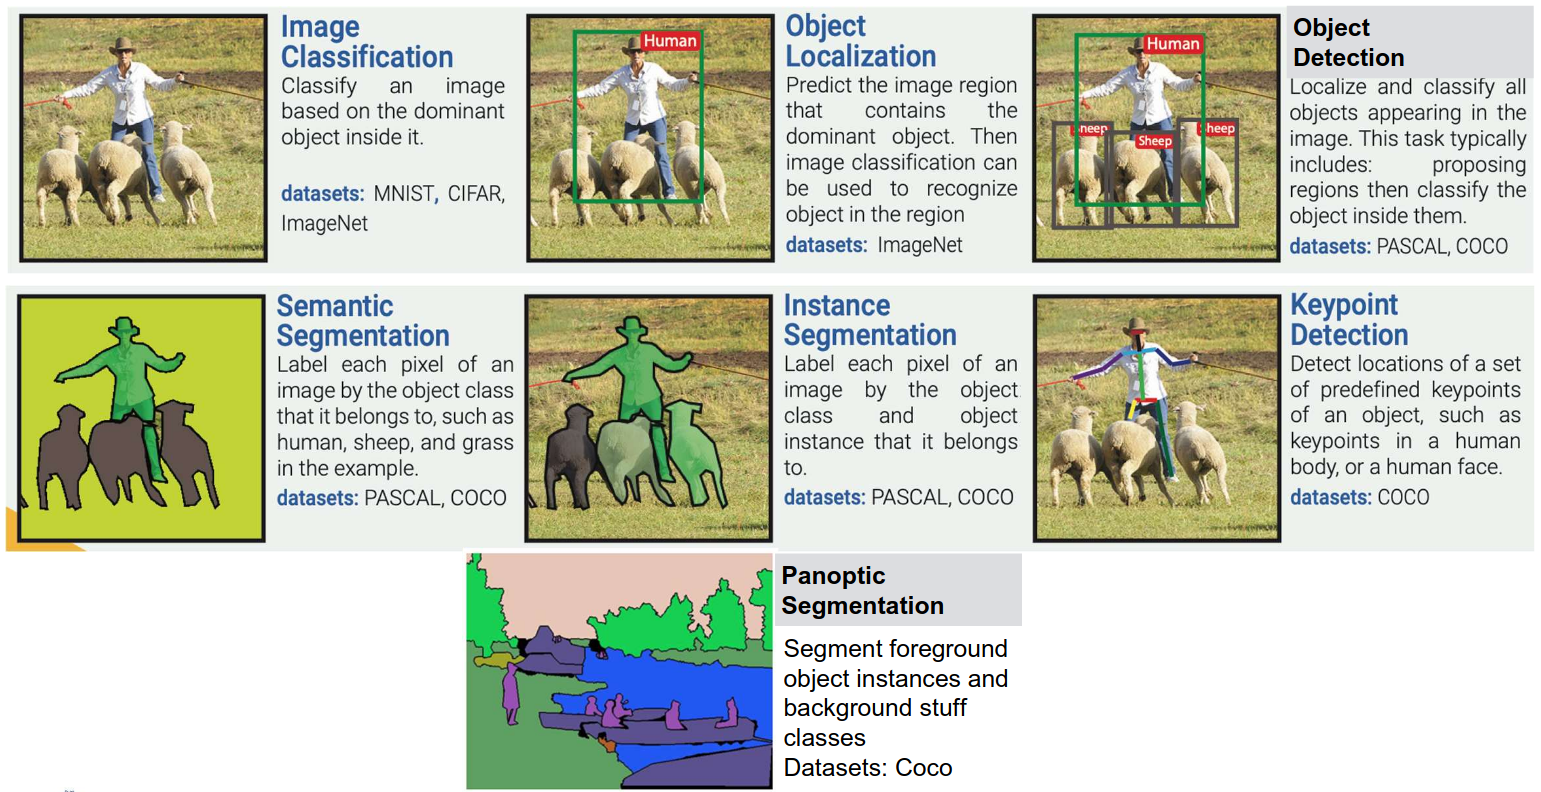
\includegraphics[width=\linewidth]{imgs/task_types.png}
\end{center}
\vspace{-1em}

\subsection{Segmentation}

\textbf{Datasets:} KITTI (only 200 training/test images), TUM SceneFlow (synthetic), City Scapes (large-scale
instance-level segmentations), COCO (Common Objects in COntext).

\vspace{-1em}
\begin{center}
    %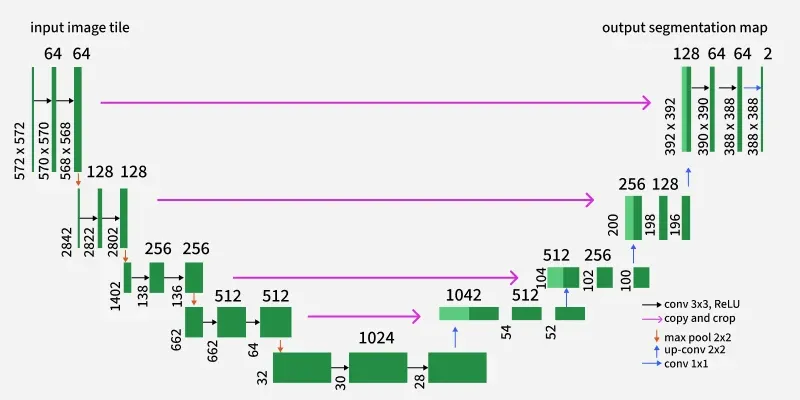
\includegraphics[width=\linewidth]{imgs/u_net.png}
    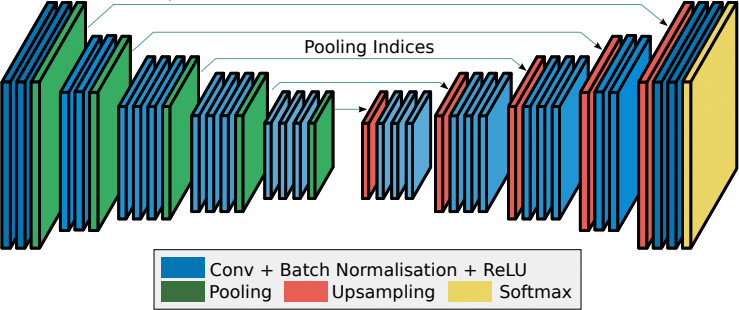
\includegraphics[width=0.8\linewidth]{imgs/segnet.png}
\end{center}
\vspace{-1em}

\textbf{Architecture:} Commonly based on U-Net or SegNet architectures, first convolutions and downsampling until a
bottleneck layer, then upsampling to recover an image with the original resolution. In U-Net upsampling is done through
upconvolutions, and there are skip connections between the upsampling and downsampling layers. In SegNet upsampling is
done through max unpooling and there are no skip connections.

\textbf{Basic Upsampling:} Replacing each cell with the value of its nearest neighbour, or leaving cells without a value
as zero (bed-of-nails).

\textbf{Max-Unpooling:} Remembering which indices had the max value during max pooling, then restoring the values at
these indices during upsampling with a bed of nails.

\textbf{Learnable Upsampling/Upconvolution:} Using a learnable kernel, multiplied by each input value and summed in the
output, giving weighted copies of the filter.

\subsection{Localization/Pose Estimation}

\textbf{PoseNet:} A CNN (GoogLeNet) for 6-DoF camera relocalization from a single image.
Loss function \(\mathcal L(I) = \norm{\hat{\bm x} - \bm x} + \beta\norm*{\hat{\bm q} - \frac{\bm q}{\norm{\bm q}}}\).
Accuracy is much worse than classical methods, but faster and uses less memory (represents map with fixed-size network).

\textbf{SfMLearner:} Unsupervised learning using photometric loss for monocular depth prediction and relative pose
prediction. Consists of a depth CNN (U-Net) and pose/explainability network (similar to SegNet). During training, depth
predictions and relative pose predictions are used to warp the current image (similar to dense/photometric mapping), and
loss compares the prediction with the actual next image. The explainability mask filters out moving objects and
occlusions; during training it also has a smoothness and regularization (encouraging nonzero predictions) term to
prevent it from masking out all points.

\textbf{Sun-BCNN:} A Bayesian CNN (GoogLeNet) for predicting the angle of the sun (and confidence) in an image, which can
be used in visual odometry to constrain the error to linear growth, without a dedicated sun sensor. Uses cosine distance
loss \(\mathcal L = 1 - \hat{\bm s}_k \cdot \bm s_k\).

\textbf{Combining Classical and Learning Based Approaches:}
\begin{enumerate}
    \item Correction: Use classical techniques to estimate a solution, then use a learning based method to apply a correction, e.g. correcting systematic bias in pose estimation.
    \item Augmentation: Using learning based methods to get additional information, then using a classical method to predict the solution with the extra information, e.g. Sun-BCNN.
    \item Initialization: Using learning methods to get an initial guess for the solution, then using classical methods to refine the solution accuracy, e.g. using PoseNet for initialization, then classic feature matching.
\end{enumerate}

\subsection{Object Localization and Detection}

\textbf{Nonmaximum Suppression:} Used to prune overlapping network outputs. First sort all predictions by confidence
score. Then for each box, starting with the highest confidence, include it in the final output set, and prune all
remaining boxes (not in the output set) whose IoU with the box we just included is over some specified threshold. Note
each class should be considered separately.

\textbf{Bounding Box/Region Proposals:} Tuples \((x, y, w, h)\) and confidence, indicating a rectangular region. Can use
simple L2 distance of the bounding box vectors as a similarity metric, or Intersection over Union (IoU) (ratio of
overlap area over total area).

\textbf{Region Proposal Methods:} Identify potential regions (\textit{anchors}) with an algorithm or region proposal
network, then for each region run region run a detector network to calculate the class scores (or background), and a
regression network to calculate a bounding box correction. Take all regions over a confidence threshold and apply NMS
for final output.
During training, loss is evaluated on all anchors instead of best ones. Take 3:1 ratio of negative to positive anchors
to avoid bias towards negative samples, choosing negatives with highest classification loss (hardest examples).

\vspace{-1em}
\begin{center}
    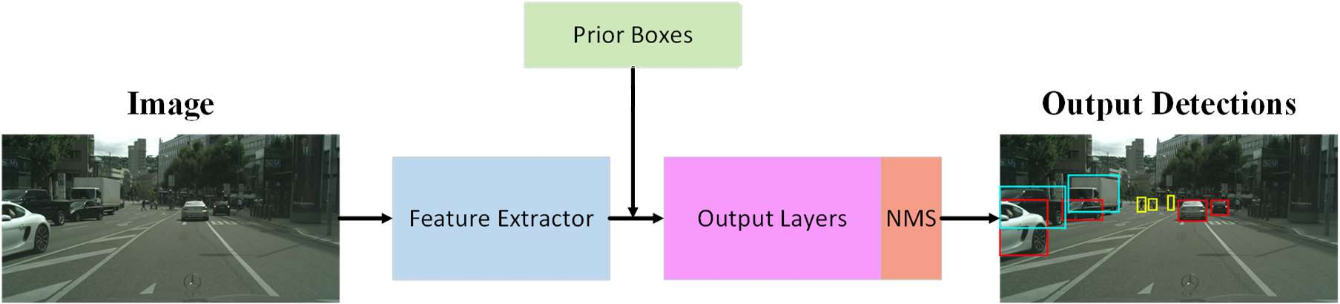
\includegraphics[width=\linewidth]{imgs/region_proposal.png}
\end{center}
\vspace{-1em}

\textbf{R-CNN:} Used classical algorithm for proposals, CNN and SVM to calculate class scores and regress bounding box
corrections.

\textbf{Fast R-CNN:} Passing the entire image through a CNN to get a feature map first, then cropping the feature map
for each proposal region.

\textbf{Faster R-CNN:} Using a learned region proposal network to generate proposals.

\textbf{Single-Shot Methods (YOLO):} Predicting bounding box coordinates and class probabilities in a single pass,
without proposals. Break the image into \(S \times S\) grid, where each cell predicts \(B\) possible bounding boxes and
confidences and \(C\) class probabilities (including background). Outputs \(S \times S \times (5B + C)\) values in
total. Multiply bounding box confidence by class probability, take the highest combined confidence for each class and
apply NMS to get final output.

Generally single-shot approaches are much faster and can run in real-time, but are slightly less accurate than proposal
based approaches.

\subsection{3D Object Detection}

\textbf{AVOD-FPN:} Generate ground-anchored proposals from both an image feature map and a birds-eye-view LiDAR feature
map, then fusing the two, performing detections in image and BEV LiDAR separately, then fusing the results again.

\textbf{Categorical Depth Distribution Network:} For monocular 3DOD, instead of generating a single depth for each
pixel, generate a depth distribution represented as a histogram instead.

\textbf{BayesOD:} Generating probabilistic uncertainty estimates instead of just confidences from 3DOD so it can be
fused with other sensors. Instead of NMS, each detection can be treated as a separate measurement for uncertainty
estimation. The network can regress a variance directly. Can also use dropout on the network during inference and
measure the difference between predictions.

\textbf{Domain Adaptation:} Transferring a detector trained on one dataset to another, e.g. adapting it for adverse
weather. Can be done through a student-teacher architecture, where the teacher provides pseudo-labels on the target
dataset to train the student with (taking only the most confident detections), and the student is taught to ignore
dataset variations (by training it to produce the same output for an original image vs. a corrupted image) while
retaining detections. Foundation models such as DINOv2 can be used in the teacher network due to their excellent domain
transfer capabilities.

\section{Application: Computer Vision on Mars} %%%%%%%%%%%%%%%%%%%%%%%%%%%%%%%%%%%%%%%%%%%%%%%%

\textbf{MER-DIMES:} Used to estimate horizontal velocity during landing of MER to determine when to fire rockets.
Inputs: radar distance to ground, monocular camera. Estimates motion over 3 frames by using 2 features and fusing with
IMU/altitude. Pipeline: Downsampling, masking shadow, determine image overlap, Harris corners, correction for CCD
effects, patch rectification, then feature matching over 2-scale pyramid.

\textbf{Spirit and Opportunity:} Used 3 sets of stereo, hazcams under solar panels for close-range obstacle detection,
navcams on main mast for visual odometry (wheel odometry insufficient due to wheel slip and degradation of calibration),
pancams for long-range panoramic imaging. Estimate traversibility by fitting planes to patches, checking for protrusions
and tilt, then inflating an occupancy grid. Even more cameras on the larger Mars Science Laboratory.

\textbf{Ingenuity Helicopter VO:} Using a single camera, RANSAC for outlier rejection and shadow removal, matching using 12 FAST
features, accounts for motion blur, lighting changes, feature-poor terrain.

\end{document}
